\chapter{実機を用いたトリガーロジックの性能評価}
\label{chap_TriggerTest}

\section{実機試験システムの概要}
\subsection{実機試験システムのコンセプト}
高輝度LHC-ATLAS実験に向けたエンドキャップ部ミューオントリガー開発は、前章までにコンセプト設計、モジュールごとのHDL設計、トリガーロジックの全体ファームウェアへの統合が完了し、ハードウェア上で論理回路を動作させるための準備が整った。次の重要なステップはトリガー回路が統合ファームウェアの中で正常に動作していること、また期待したトリガー性能を実現できていることを検証することである。

しかし、一般に、ハードウェア上で動作する大規模トリガー回路を実験開始前の段階で試験するには工夫が必要となる。SLでもトリガー回路の入力はPS boardから受信する光信号、出力はFELIXに送信する光信号で、このままではPS boardやFELIX、さらに後段の読み出し回路が完成するまで、試験をするすべがない。

そこで本研究では、SoCを活用した次世代的なシングルボード試験システムを開発した。図\ref{Concept_test}にそのコンセプトを示す。

\begin{figure} 
\centering
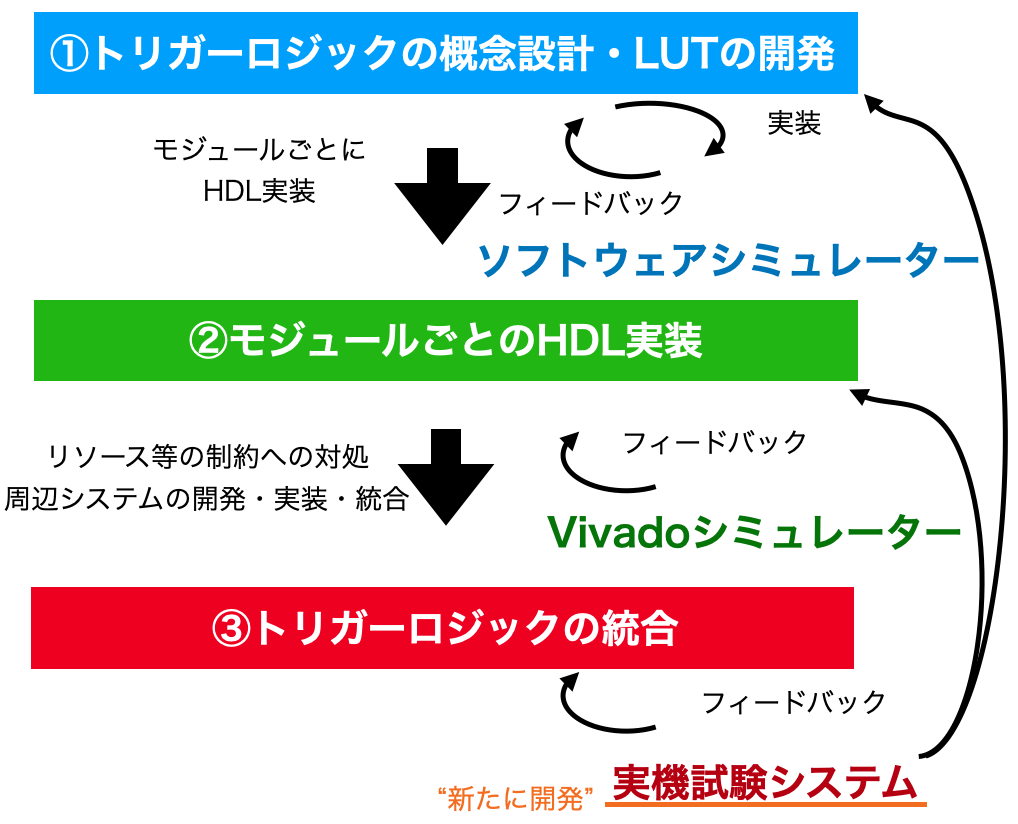
\includegraphics[width=16cm]{fig/Test/Concept_test.png}
\caption[実機試験システムのコンセプト]{実機試験システムのコンセプト。新しく開発する実機試験システムは統合したトリガーロジックに対する検証システムとして働くだけでなく、}
\label{Concept_test}
\end{figure}

このシステムでは、モンテカルロシミュレーションデータや実データなど任意のデータセットをハードウェア上のロジックに投入し、実際のトリガー演算結果を自由に取り出すことができる。LUTの書き込みやTTC信号の分配、トリガー読み出しなどはSLの本番運用と同じものを利用するため、統合ファームウェア全体の動作検証にもつながる。さらに、トリガーロジック自体に対する検証としても、ソフトウェアシミュレーター、Vivado シミュレーターより、本番に即した試験を実現する。図\ref{Test_Flow}にこれまでの試験と、本システムで達成する試験フローの違いを示す。

\begin{figure}
    \begin{minipage}[b]{0.9\linewidth}
    \centering
    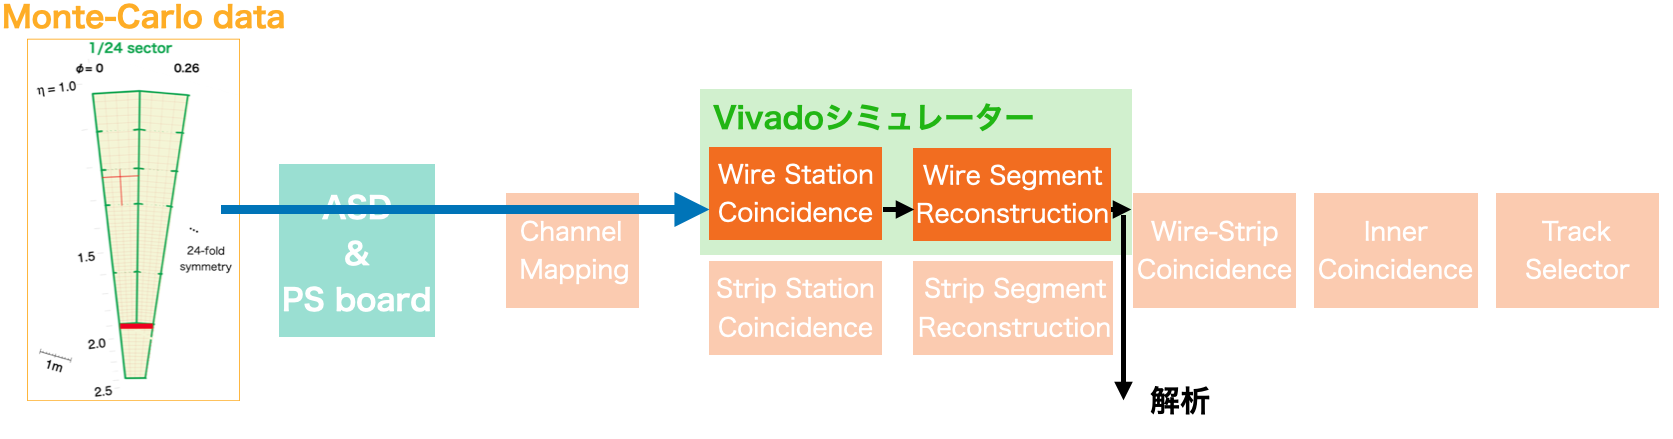
\includegraphics[height=4.8cm]{fig/Test/Flow_Wire.png}
    \subcaption{Vivadoシミュレーターによる試験フロー : Wire Segment Reconstruction}
    \end{minipage}\\
    \begin{minipage}[b]{0.9\linewidth}
        \centering
        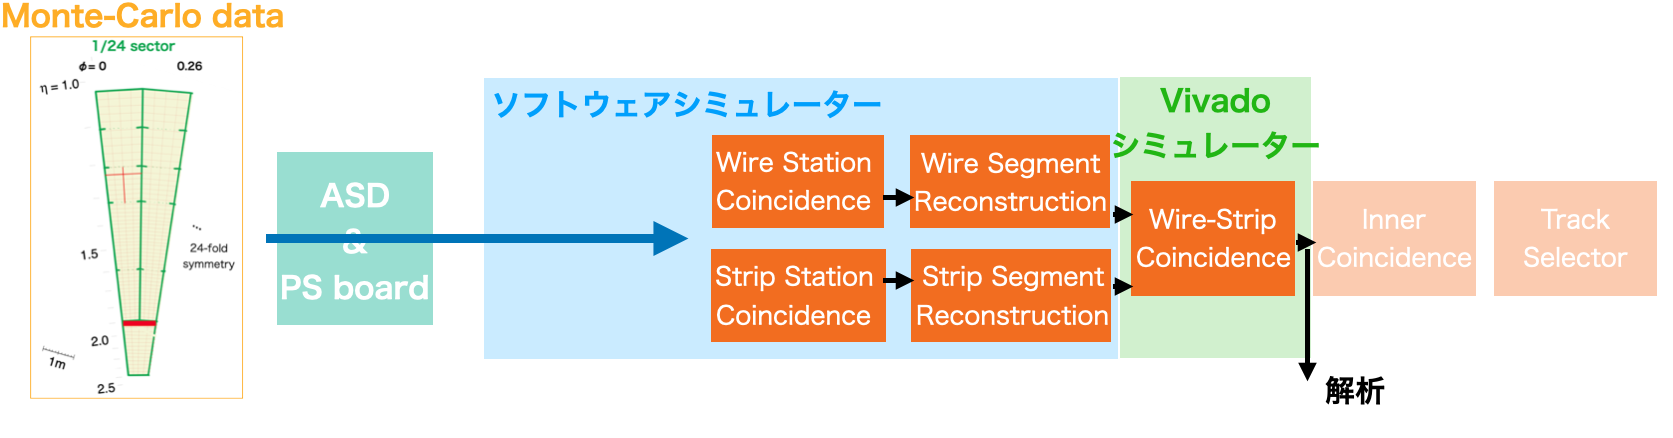
\includegraphics[height=4.8cm]{fig/Test/Flow_WS.png}
        \subcaption{Vivadoシミュレーターによる試験フロー : Wire Strip Coincidence}
    \end{minipage}\\
        \begin{minipage}[b]{0.9\linewidth}
            \centering
            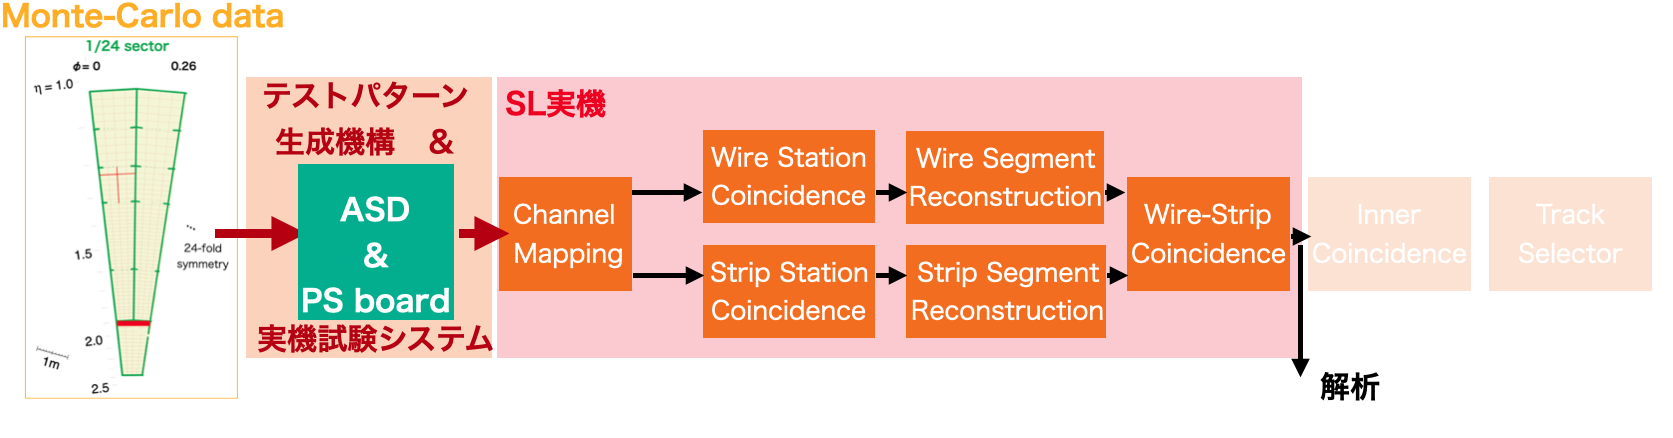
\includegraphics[height=4.8cm]{fig/Test/Flow_zikki.png}
            \subcaption{実機試験システムによる試験フロー}
        \end{minipage}\\
    
    \caption[試験フロー]{Vivado シミュレーター、ソフトウェアシミュレーターによる試験フローと実機試験フローの比較。}
    \label{Test_Flow}
\end{figure}

これまではMCサンプルやソフトウェアシミュレーターから、各モジュールのインプットを生成し、モジュール単位でVivadoシミュレーションを回していた。本システムではTGCのヒット情報から、フロントエンドエレクトロニクスの複雑な配線情報も考慮した上で、PS boardからSLに送られる8,000 bitのヒット情報を完全に再現し、トリガーロジックのインプットとする。これによりChannnel Mapping、Station Coincidence、Segment Reconstruction、Wire Strip Coincidenceと接続されたトリガーモジュールをフルチェーンで試験することができる。また、ソフトウェアシミュレーターではパターンマッチング用のLUTは最終出力のテキストファイルではなく、もととなるrootファイルを利用する。本試験ではいくつかの処理を経て、最終的に出力された本番で使われるテキストファイルを利用するためLUTの最終検査も行うことができる。さらに実機試験システムはトリガー演算をFPGA上で行っているため、Vivado シミュレーターと比べて高速で動作する。これにより、大統計を活かした網羅的な検証が可能で、これまでVivado シミュレーターでは発見することができなかった局所的なHDLのバグの発見も期待される。\footnote{Vivado シミュレーターはデジタル回路の全ての信号遷移をソフトウェア的に計算するため、回路規模が大きくなると動作が遅くなる。ファームウェア全体をシミュレーションすると、数10イベントに半日程度かかることがわかっており、高統計の試験はできなかった。}

次節に実機試験システムの全体像を説明する。

\subsection{実機試験システムの全体像}
\label{subsec_TestSystemOverview}
図\ref{Test_system}に実機を用いた試験システムの全体像を示す。このシステムは主にテストパターン生成システム、実機試験システム、Bit-wiseシミュレーターで構成される。実機試験システムは本研究で開発を進めた。テストパターン生成システムおよびBitwiseシミュレーターは先行研究で開発された。以下にそれぞれの詳細を説明する。

\begin{figure} 
\centering
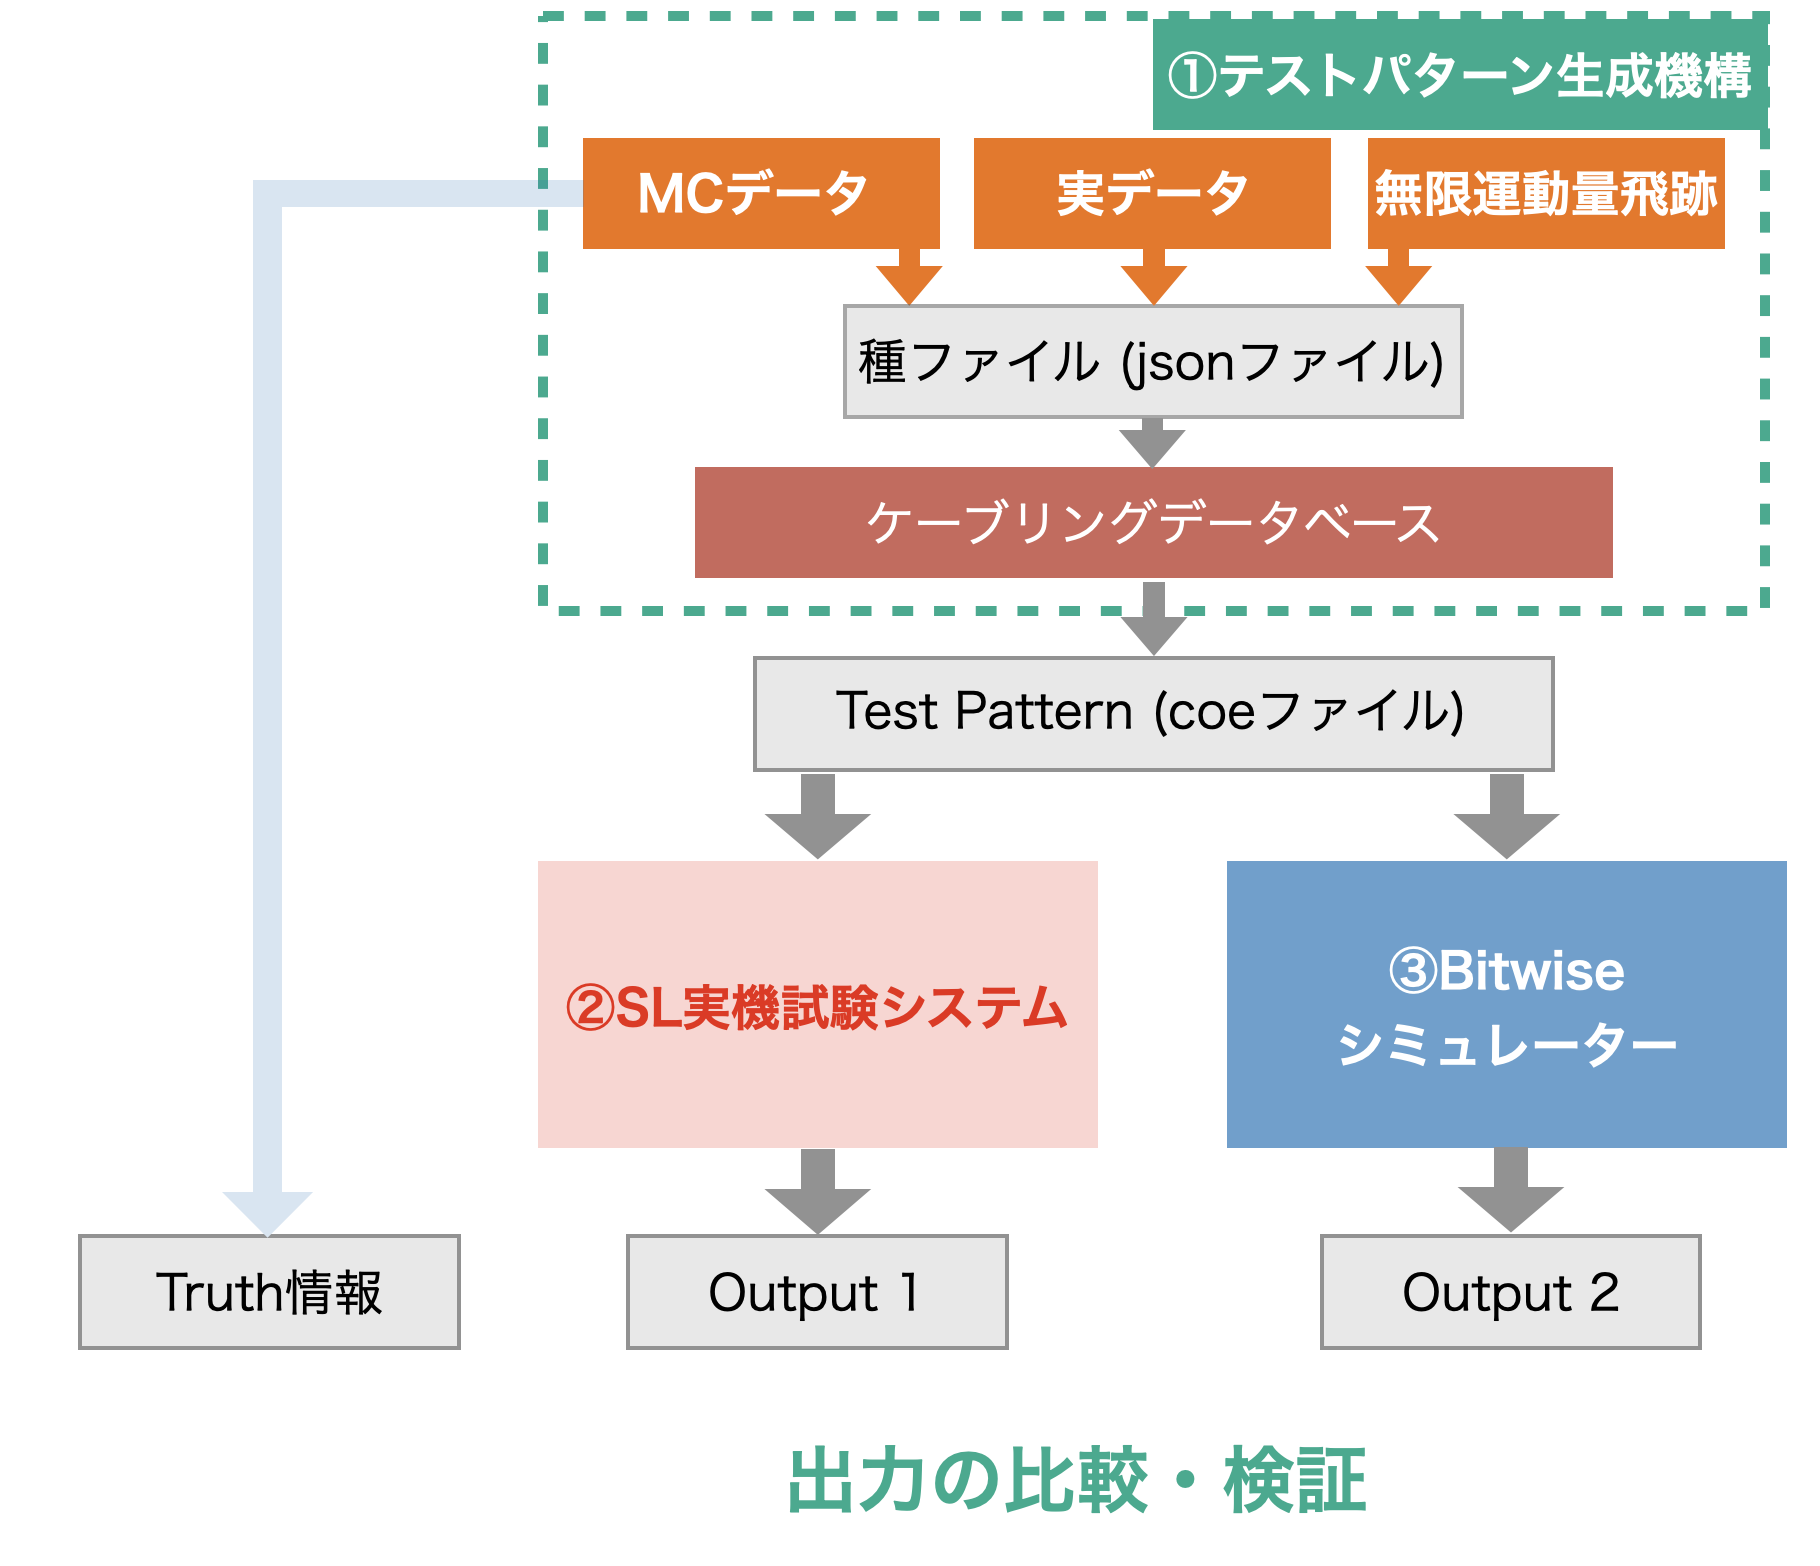
\includegraphics[width=16cm]{fig/Test/Test_system.png}
\caption[実機試験システムの概要]{実機試験システムの概要}
\label{Test_system}
\end{figure}

\paragraph{テストパターン生成システム}  
\par
\ref{chap_TGC}節で述べたようにSLは、1枚のPS boardから2本の光ファイバーを通じて128 bit x 2 ファイバーのヒット信号を受け取る。1枚のSLは合計 31枚のPS boardと接続するため、イベントごとに128 bit x 62 ファイバーのヒットビットマップがトリガーロジックに入力される。モンテカルロシミュレーションや過去のRunで取得された、TGCのヒットチャンネルの情報から、トリガーロジックに入力されるヒットビットマップをエミュレートする仕掛けが、テストパターン生成システムである。

テストパターン生成システムは、元のデータセットに格納されている、各イベントにおけるTGC検出器のチャンネルごとのヒット情報を抽出し、テストパターンの種ファイルとしてjsonファイルに格納する。この際、モンテカルロデータ、実データ、toyデータなどいかなるデータセットも統一的なフォーマットでjsonファイルを作成することで、この後の処理はその違いに関わらず進めることができる。生成されたjsonファイルはケーブリングデータベースと接続される。ケーブリングデータベースはTGC検出器からSLまでの複雑な配線情報 (ASD、PS board、SLと続く物理的なケーブルの配線に加え、各デジタル回路内の信号の並び替え情報等も含む) を一元的に管理しているデータベースである。この2つを合わせることで、任意のデータセットからSLのインプットを再現したテストパターンを生成することができる。テストパターンはSL実機、Vivado シミュレーション、後述するBitwiseシミュレーターに共通して入力できるようにcoeファイル形式で出力される。これにより、全く同じインプットを入力に用いた、コヒーレントな検証が可能になっている。

\paragraph{実機試験システム}  
\par
実機試験システムは生成されたテストパターンをインプットに、実際にハードウェア上でトリガー回路を動作させ、その出力を取り出すシングルボード試験システムである。その詳細は次節説明する。

\paragraph{Bitwiseシミュレーター}  
\par
BitwiseシミュレーターはSLトリガーロジックをビットレベルで再現したC++ベースのシミュレーターである。このシミュレーターはテストパターンを入力とし、LUTもテキストファイルとしてダンプされた最終生成物を使用するため、実機システムと完全に同じ道具を利用してシミュレーションを行う。そのため、実機システムとの比較・検証用に極めて有用である。また、各モジュールのロジックや入出力もファームウェアと完全に一致するように設計されているため、途中出力同士の比較や、実機出力では出せない内部の信号線の調査にも利用することができ、HDLの精密なデバッグが可能である。\footnote{前述のソフトウェアシミュレーターは実現しているロジックはファームウェアと完全に等価であるが、入力データやLUTは実機システムとは異なるため、最終的な動作確認には不向きである。また内部でビットレベルの演算を行なっている訳ではないので、途中出力をファームウェアと比較することもできない。}

\section{実機試験システムの開発}
\subsection*{ファームウェアの概要}
本節では、トリガー回路の試験用に開発したシングルボード試験システムについて説明する。
図\ref{TestSystem_Overview}に実装したトリガーロジック試験システムの概要を示す。試験システムのコントロールおよびデータ読み出しはMPSoC上のLinuxを起点に行う。本システムではSL単体での試験を実現するため、SL上の水晶発振器で生成した40.079 MHzクロックをLHC陽子バンチ交差クロックの代わりに基準クロックとして扱う。FELIXから配られるTest Pulse Trigger (TPT)やL0AなどのTTC信号もSL内部のTTC emulatorで擬似的に生成し、各モジュールに分配する。

\begin{figure} 
\centering
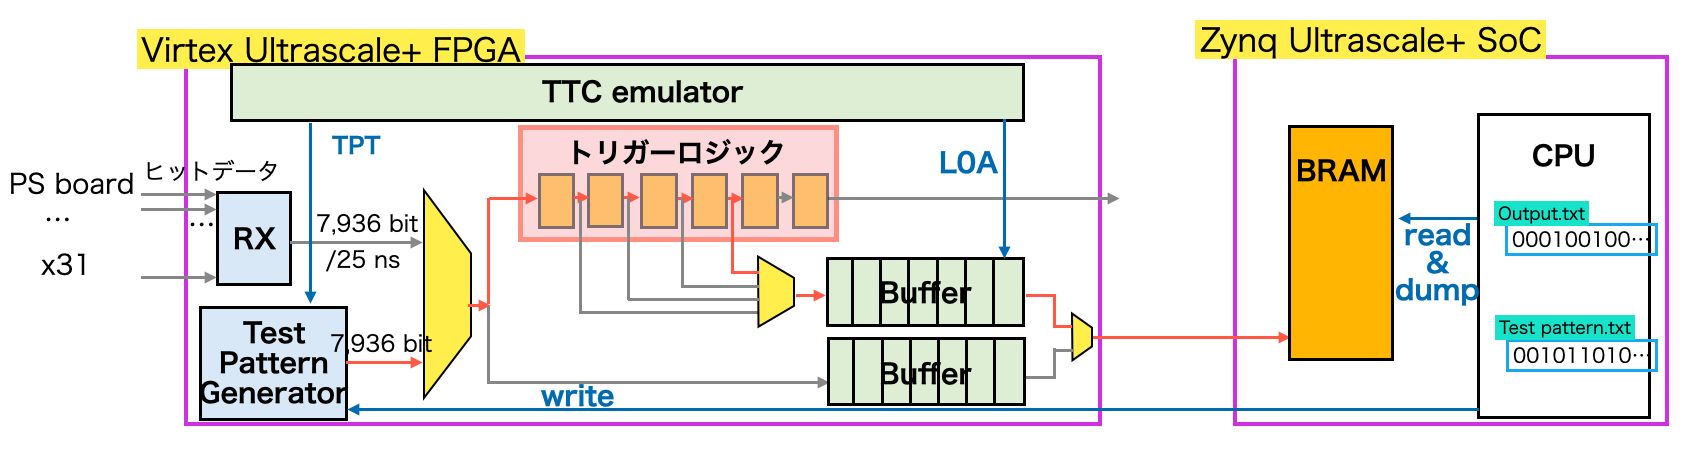
\includegraphics[width=16cm]{fig/Test/TestSystem_overview.png}
\caption[トリガー試験ファームウェアの概要]{トリガー試験ファームウェアの概要}
\label{TestSystem_Overview}
\end{figure}

PS boardから受信するヒット信号をエミュレートしたテストパターンは、Test Pattern Generator内のBRAMに格納される。Test Pattern GeneratorはTTC emulatorからTest Pulse Trigger (TPT) 信号を受信すると、1イベント分のヒットビットマップをトリガー回路に投入する。Trigger Logicからの出力はLHCバンチ交差クロックに同期してL0 Bufferにダンプされ、読み出し回路を経てMPSoC上のLinuxから読み出される。トリガー回路は固定レイテンシーで動作するため、TTC emulatorはTPTから決まったクロックチック後にL0Aを出すことで、TPTに該当するトリガー出力を読み出すことができる。以下に各モジュールの概要を説明する。

\paragraph{Test Pattern Generator}  
\par
Test Pattern Generator は幅 128 bit、深さ 64 のBRAMで、1つのBRAMがPS board 1リンク分の信号をエミュレートする。全31 PS board $\times$ 2リンクの信号をエミュレートするために合計62個のBRAMが並列に配置されている。トリガーロジックの入力としてTest patternを入力するか、PS boardから受信したデータを入れるかはスイッチで切り替えられるようになっている。テストパターンはcoe形式のファイルを用いてBRAMの初期値として設定することができる。さらにMPSoCから何度でも上書きすることができるため、BRAMの深さ64に制限されることなく、任意のイベント数で試験することができる。

\paragraph{トリガーロジック}  
\par
トリガー回路の出力は読み出し用のフォーマットに整形され、トリガー読み出し回路へ渡される。今回の試験では各モジュールの動作を詳細に調査するため、モジュール間で受け渡される全てのビットマップを読み出せるようフォーマットを定義している。例としてWire Strip Coincidenceの読み出しデータを説明する。Wire Strip Coincidenceは44の8 regionと34の32 regionで構成され、160 MHzクロックに同期して、8regionから最大1つ、32 regionから最大4つのミューオン候補がInner Coincidenceに送られる。読み出し回路でもこの最大180のミューオン候補を並列に読み出せるよう設計しており、各領域ごとに表\ref{tab:WS_format}の形式にデータを整形し読み出し回路に送信する。各モジュールの出力フォーマットでは最上位1bitはvalid信号を定義するようにする。後述の読み出し回路ではこのvalid信号が立てられているユニットの出力だけを読み出すように設計しており、効率的にデータ量を削減している。

\begin{table}[]
    \centering
    \caption[Wire Strip Coincidenceの読み出しフォーマット]{Wire Strip Coincidenceの読み出しフォーマット。}
    \label{tab:WS_format}
    \begin{tabular}{|c|c|}
    \hline
    \# of bits & Name                                                                                        \\ \hline\hline
    1          & The flag indicates that the region has received at least one wire segment and strip segment \\ \hline
    4          & $p_{\mathrm{T}}$ threshold reconstructed using Coincidence                                  \\ \hline
    3          & Reserved                                                                                    \\ \hline
    7          & $\Delta\theta$ from Wire Segment Reconstruction                                             \\ \hline
    2          & Number of stations with the hits used for wire segment                                      \\ \hline
    4          & $\Delta\phi$ from Strip Segment Reconstruction                                              \\ \hline
    2          & Number of stations with the hits used for strip segment                                     \\ \hline
    1          & Reserved                                                                                    \\ \hline
    \end{tabular}
\end{table}


それぞれのトリガーモジュールから読み出すデータの出力ビット幅を表\ref{tab:output_width}に示す。ビット幅の大きな出力を後段の読み出しロジックに一斉にダンプすると、タイミング制約を満たすことが難しくなるため、そのような出力はいくつかの並列なレーンに分割して処理している。

\begin{table}[]
    \centering
    \caption[各モジュールの出力ビット幅]{各モジュールの出力ビット幅。}
    \label{tab:output_width}    
    \begin{tabular}{|c|c|c|c|}
    \hline
    トリガーロジック                                      & SLR & 出力ビット幅 (bits) & レーン数 \\ \hline\hline
    \multirow{3}{*}{Channel Mappin}               & 0   & 2732          & 4    \\ \cline{2-4} 
                                                  & 2   & 2732          & 4    \\ \cline{2-4} 
                                                  & 3   & 1000          & 2    \\ \hline
    \multirow{3}{*}{Wire Station Coincidence}     & 0   & 1768          & 3    \\ \cline{2-4} 
                                                  & 2   & 1768          & 3    \\ \cline{2-4} 
                                                  & 3   & 804           & 3    \\ \hline
    \multirow{3}{*}{Strip Station Coincidence}    & 0   & 1890          & 3    \\ \cline{2-4} 
                                                  & 2   & 1890          & 3    \\ \cline{2-4} 
                                                  & 3   & 378           & 3    \\ \hline
    \multirow{3}{*}{Wire Segment Reconstruction}  & 0   & 3404          & 5    \\ \cline{2-4} 
                                                  & 2   & 3404          & 5    \\ \cline{2-4} 
                                                  & 3   & 1472          & 2    \\ \hline
    \multirow{3}{*}{Strip Segment Reconstruction} & 0   & 360           & 1    \\ \cline{2-4} 
                                                  & 2   & 360           & 1    \\ \cline{2-4} 
                                                  & 3   & 72            & 1    \\ \hline
    \multirow{3}{*}{Wire Strip Coincidence}       & 0   & 1776          & 3    \\ \cline{2-4} 
                                                  & 2   & 1776          & 3    \\ \cline{2-4} 
                                                  & 3   & 768           & 1    \\ \hline
    \end{tabular}
\end{table}

全てのトリガーロジックの読み出し回路を同時に実装するのはリソースの観点で不可能である。読み出したいデータをリンクごとに選択し、目的に応じて異なるファームウェアを用意して試験を行う。例えばFW領域のロジックを重点的に調べたい場合には、SLR3のStation CoincidenceからWire Strip Coincidenceまでのリンクを選択する。一方、全トリガーセクターにおける特定のモジュールを出力させる、などのカスタマイズも可能である。実験本番で用いるファームウェアでは、各トリガーロジックからの出力から必要最低限な情報を抜き出すことで、全てのトリガーモジュールの出力を同時にモニターする。

\paragraph{トリガー読み出し回路}  
\par
トリガー読み出し回路はトリガーモジュールの出力をMPSoCから読み出すための仕掛けである。図\ref{Readout_Circuite}に読み出し回路の概要を示す。以下に各モジュールの役割を説明する。

\begin{figure} 
\centering
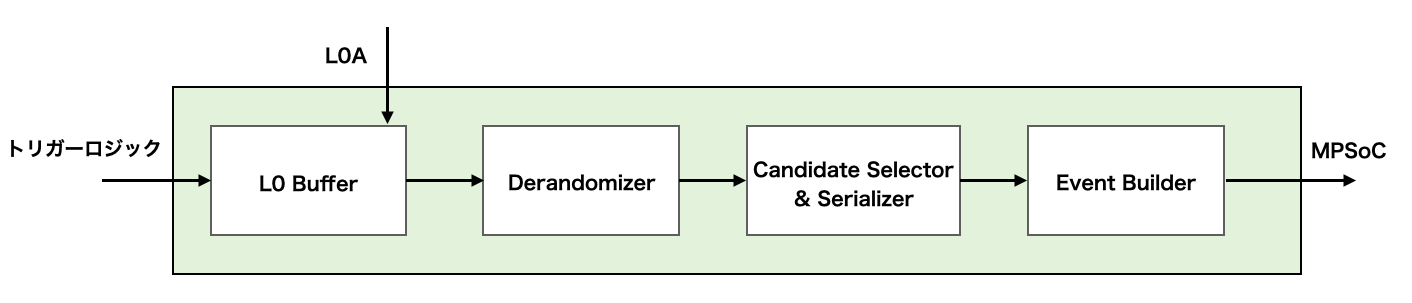
\includegraphics[width=16cm]{fig/Test/Readout_Circuite.png}
\caption[トリガー読み出し回路の概要]{トリガー読み出し回路の概要}
\label{Readout_Circuite}
\end{figure}

\begin{itemize}
    \item L0 Buffer  
    \par
    トリガーロジックでフォーマットされたデータはL0 Bufferにダンプされる。L0 Bufferは入力ビットマップと同じ幅をもつ深さ512のBRAMあり、TTC emulatorからL0Aが出されるまでのバッファリングを行う。トリガーロジックには40 MHz、160 MHz、240 MHzで駆動するものが存在する。いずれの場合でも1つの陽子バンチ衝突由来の出力は25 nsごとに横並びに揃えられ、40 MHzのLHC クロックで動作する書き込みポインタに従って、L0 Bufferに格納される。一方、読み出しは240 MHzで行われ、読み出されたデータはDerandomizerに送られる。

    \item Derandomizer  
    \par
    Derandomizerは入力ビットマップと同じbit幅をもつ深さ 512 のFIFOで、後段で行われる圧縮およびシリアル化の処理待ち用バッファーである。L0Aがアサートされたイベントをダンプし、Candidate Selector から読み出し命令が出された場合に、先頭のイベントを読み出す。

    \item Candidate Selector \& Serializer  
    \par
    Candidate Selectorは各トリガーモジュールのすべてのユニットから出力される飛跡候補の中から、ミューオン候補を再構成できたユニットの出力のみを選択して後段に送る。これにより大幅なデータ削減が達成される。選択された飛跡情報は、どのサブユニットからの出力かを示す6 bitの識別IDと2bit のbunch tagが付与され、32 bit幅のワードとして後段のSerializerに送信される。
    Serializerは32 bit幅のワードをクロックチックごとに1ワードずつ処理し、あるL0Aに対応する1イベント分のパケットをまとめて、後段のEvent Builderに渡す。図\ref{tab:packet_format}にパケットのフォーマットを示す。パケットにはイベント境界を示すための特別なワード Start of Event (SOE)、End Of Event (EOE) が挿入される。

\begin{itembox}{後で直すところ}
    表はみだし問題
\end{itembox}

    \begin{table}
        \centering
        \caption[パケットのフォーマット]{SerializerからEvent Builderに送られるパケットのフォーマット}
        \label{tab:packet_format}
        \begin{tabular}{|c|cccccccccccccccccccccccccccccccc|}
        \hline
                & \multicolumn{1}{c|}{31} & \multicolumn{1}{c|}{30} & \multicolumn{1}{c|}{29} & \multicolumn{1}{c|}{28} & \multicolumn{1}{c|}{27} & \multicolumn{1}{c|}{26} & \multicolumn{1}{c|}{25} & \multicolumn{1}{c|}{24} & \multicolumn{1}{c|}{23} & \multicolumn{1}{c|}{22} & \multicolumn{1}{c|}{21} & \multicolumn{1}{c|}{20} & \multicolumn{1}{c|}{19} & \multicolumn{1}{c|}{18} & \multicolumn{1}{c|}{17} & \multicolumn{1}{c|}{16} & \multicolumn{1}{c|}{15} & \multicolumn{1}{c|}{14} & \multicolumn{1}{c|}{13} & \multicolumn{1}{c|}{12} & \multicolumn{1}{c|}{11} & \multicolumn{1}{c|}{10} & \multicolumn{1}{c|}{9} & \multicolumn{1}{c|}{8} & \multicolumn{1}{c|}{7} & \multicolumn{1}{c|}{6} & \multicolumn{1}{c|}{5} & \multicolumn{1}{c|}{4} & \multicolumn{1}{c|}{3} & \multicolumn{1}{c|}{2} & \multicolumn{1}{c|}{1} & 0 \\ \hline
        SOE       & \multicolumn{5}{c|}{rsvd}                                                                                                       & \multicolumn{4}{c|}{data loss flag}                                                                   & \multicolumn{12}{c|}{0xB0E}                                                                                                                                                                                                                                                                                           & \multicolumn{11}{c|}{L0ID}                                                                                                                                                                                                                                   \\ \hline
        EOE       & \multicolumn{5}{c|}{rsvd}                                                                                                       & \multicolumn{4}{c|}{data loss flag}                                                                   & \multicolumn{12}{c|}{0xB0E}                                                                                                                                                                                                                                                                                           & \multicolumn{11}{c|}{L0ID}                                                                                                                                                                                                                                   \\ \hline
        data word & \multicolumn{6}{c|}{Unit address}                                                                                                                         & \multicolumn{2}{c|}{BC tag}                       & \multicolumn{24}{c|}{bitmap}                                                                                                                                                                                                                                                                                                                                                                                                                                                                                                                                                                                   \\ \hline
        buffer    & \multicolumn{12}{c|}{0xBFF}                                                                                                                                                                                                                                                                                           & \multicolumn{9}{c|}{rsvd}                                                                                                                                                                                                               & \multicolumn{11}{c|}{L0ID}                                                                                                                                                                                                                                   \\ \hline
        \end{tabular}
    \end{table}

    \item Event Builder  
    \par
    上述のCandidate Selectorまでは読み出しレーンごとに処理が行われる。Event Builderはこれらの並列なレーンの出力を直列化し、MPSoCに送信するためのフォーマットに整形し直す。Serializerから受信する32 bitのワードはEvent Builder内の処理待ちバッファーに格納される。Event Builderは処理待ちバッファーのデータを240 MHzのクロックチックごとに1ワードずつ図\ref{TriggerReadout_format}のフォーマットに整形する。meta switchは読み出しを行うトリガーロジックの選択状態を表す。meta dataは各トリガーロジックごとに送られ、そのトリガーロジックのラベル(data flavor)、読み出しを行うbunch tag ( previous, current, next, next to next )の選択状態を表す。
    実機試験ではこのようにFPGA内でエンコードされたデータを、ソフトウェア上で逐次的にデコードすることで、トリガーロジックからの出力を一意に再構成して、テキストファイルにダンプする。

    \begin{figure} 
    \centering
    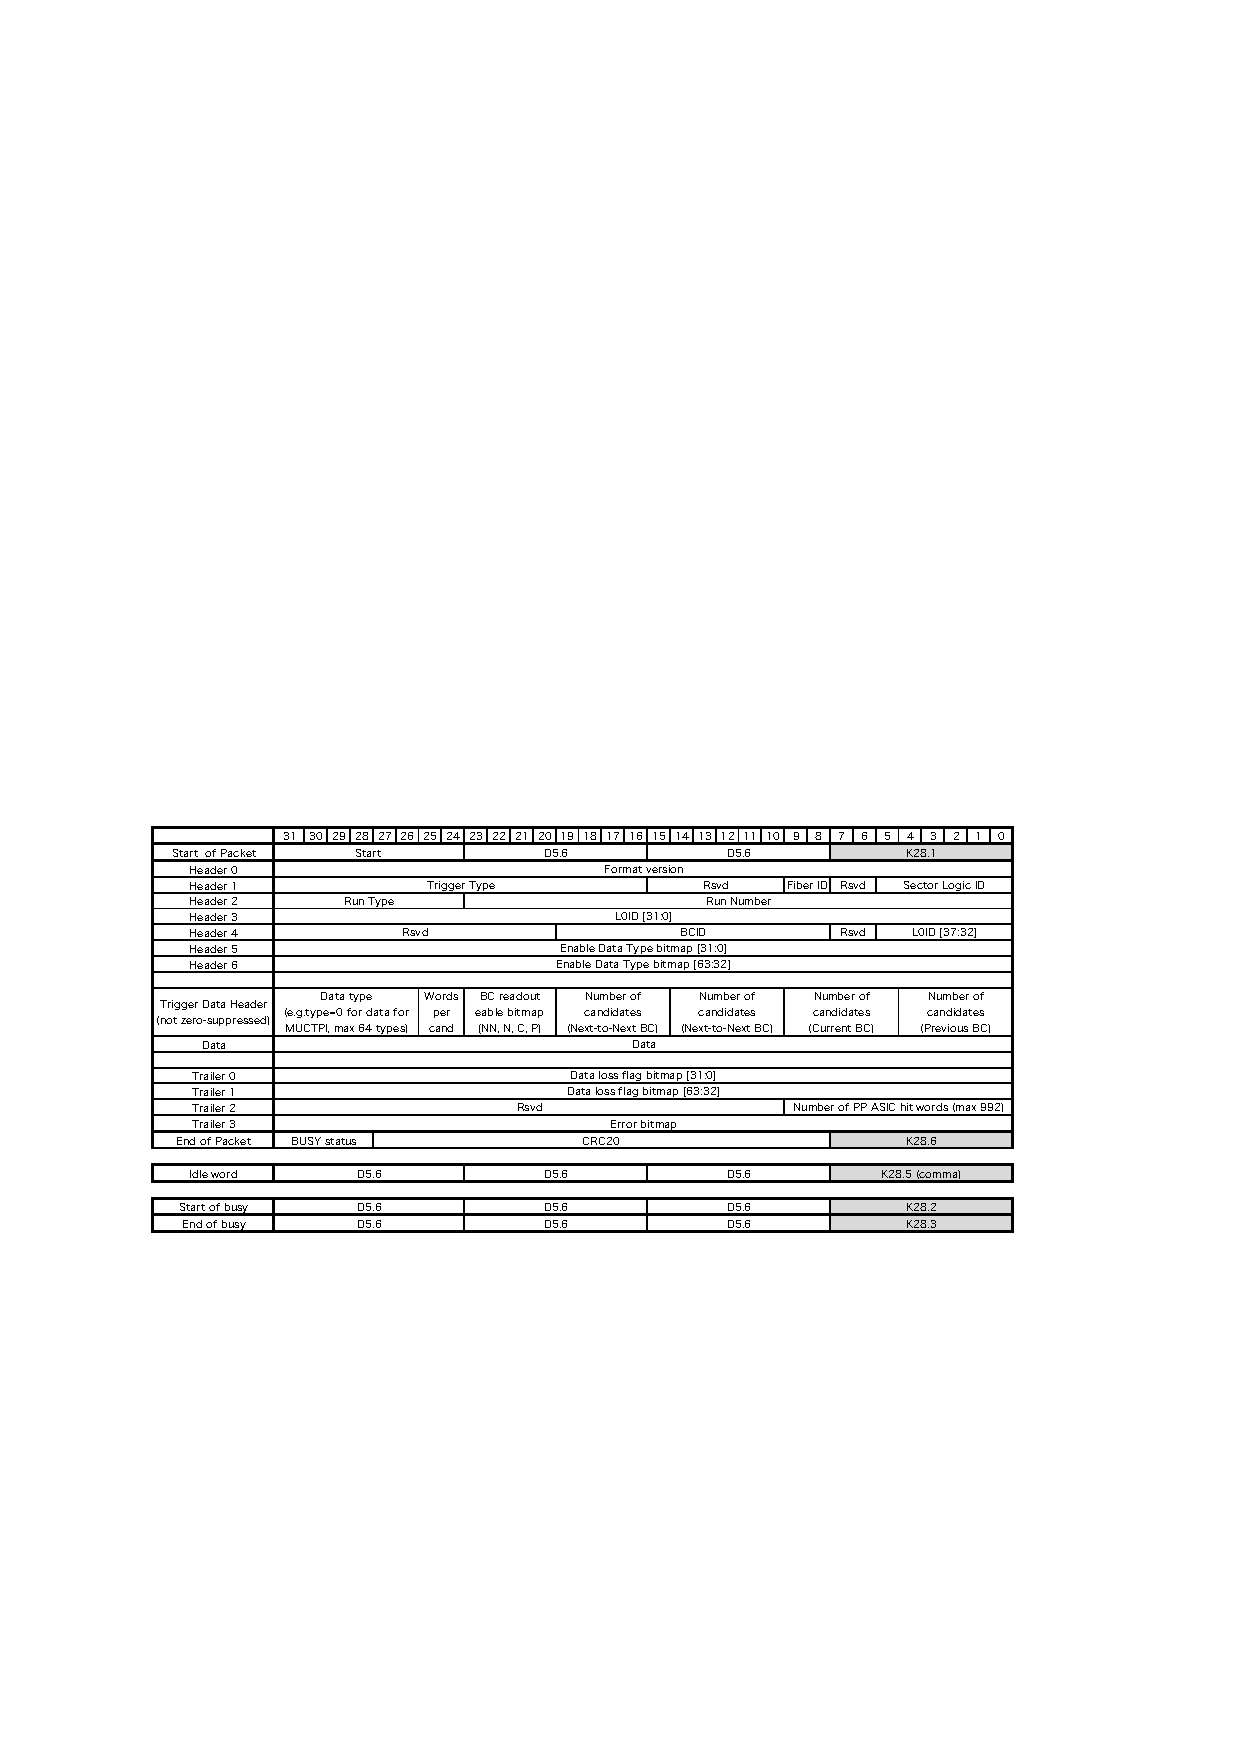
\includegraphics[width=16cm]{fig/Test/TriggerReadout_format.pdf}
    \caption[Event Builderで整形されるトリガー出力のフォーマット]{Event Builderで整形されるトリガー出力のフォーマット\cite{SLPDR}}
    \label{TriggerReadout_format}
    \end{figure}
\end{itemize}

\paragraph{SL FPGAからMPSoCへのデータ転送}  
\par
SL FPGAで整形されたデータはMPSoC PL領域内のBRAMに格納されたのち、PSから読み出される。SL FPGAからMPSoCへのデータ転送は、高速シリアル通信を利用する。図\ref{C2C}にチップ間通信の概要を示す。
\begin{figure} 
\centering
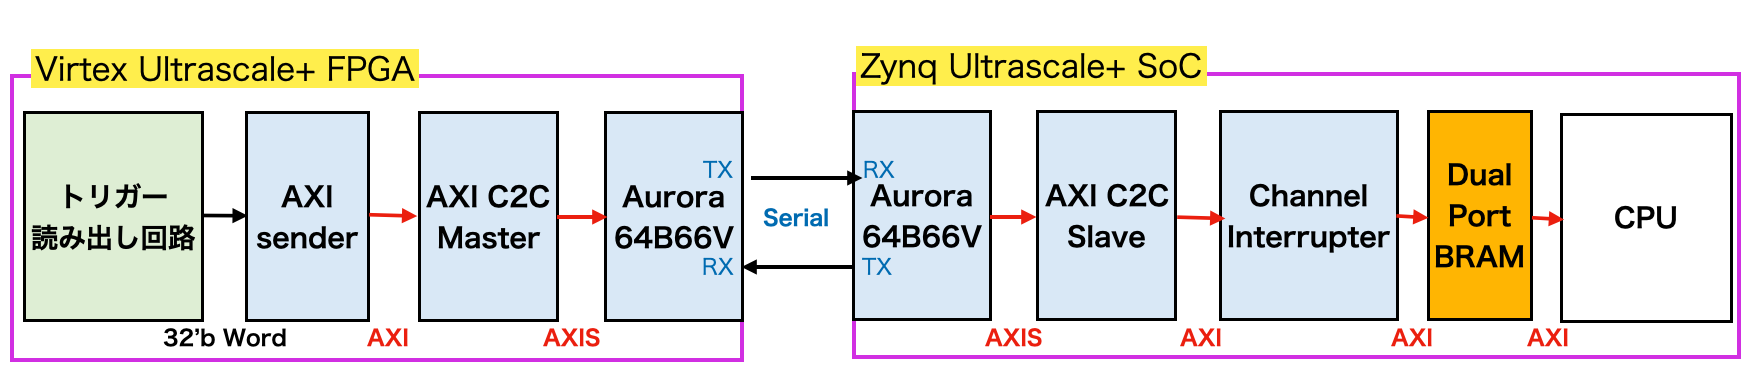
\includegraphics[width=16cm]{fig/Test/C2C.png}
\caption[SL FPGAからMPSoCへのチップ間通信]{SL FPGAからMPSoCへのチップ間通信}
\label{C2C}
\end{figure}

Event Builderから出力される32 bit幅のワードはAXI senderに送られる。AXI senderは受信したデータをデータ幅32 bit、アドレス幅 32 bitのバス通信であるAXIプロトコルで、AXI chip2chipへ送る。AXI chip2chipはAXI形式のデータをAXI Stream 形式に変換し、Aurora 64B/66B Masterと通信する。AXI chip2chip以降のデータ転送ではAXIバーストと呼ばれる、連続したデータブロックを高速転送するための手法が採られている。AXIバーストはMasterからSlaveに送信するワード数を事前に定義 ( 本システムでは256ワード ) することで、通常のハンドシェイキングで生じるバスのアイドルタイムを最小限にすることができる。
Aurora 64 B/66B MasterはAXI Stream形式のデータをシリアル通信のデータにエンコードし、ギガビットトランシーバーを用いてチップ間通信を行う。

シリアルデータは、MPSoCのPLに実装されたAurora 64B/66B Slaveで受信され、再びAXI Stream形式にデコードされた後、AXI chip2chip でAXI 形式へと変換される。MPSoCでAXI形式に戻されたデータはChannel Interrupterを中継して、幅32bit、深さ8192 のdual port BRAMにダンプされる。BRAMのもう片方のポートはMPSoCのPSにAXI形式で接続されており、BRAMを介してPLからPSへのデータ送信が可能になっている。AXIバーストを利用していることで1イベント当たりのワード数は256に固定されている。BRAMには最大$ \,8192 / 256 = 32\,$ イベント分のデータを格納することができる。一度BRAMがfullになったら、MPSoCからマニュアルでリセットをかけることで、データ取得を再開できる。

\paragraph{アプリケーション}  
\par
シングルボードのトリガー試験を行うために開発した、MPSoC上で走るアプリケーションの概要を説明する。このアプリケーションはSLのSDカード上にテキストファイルとして保存されたLUTやテストパターンをハードウェアに書き込み、テストパルスをトリガーし、トリガーの演算結果をBRAMから読み出し、デコードしたデータをSDカード上のテキストファイルにダンプする。
図\ref{Flowchart}にアプリのフローチャートを示す。

\begin{figure} 
\centering
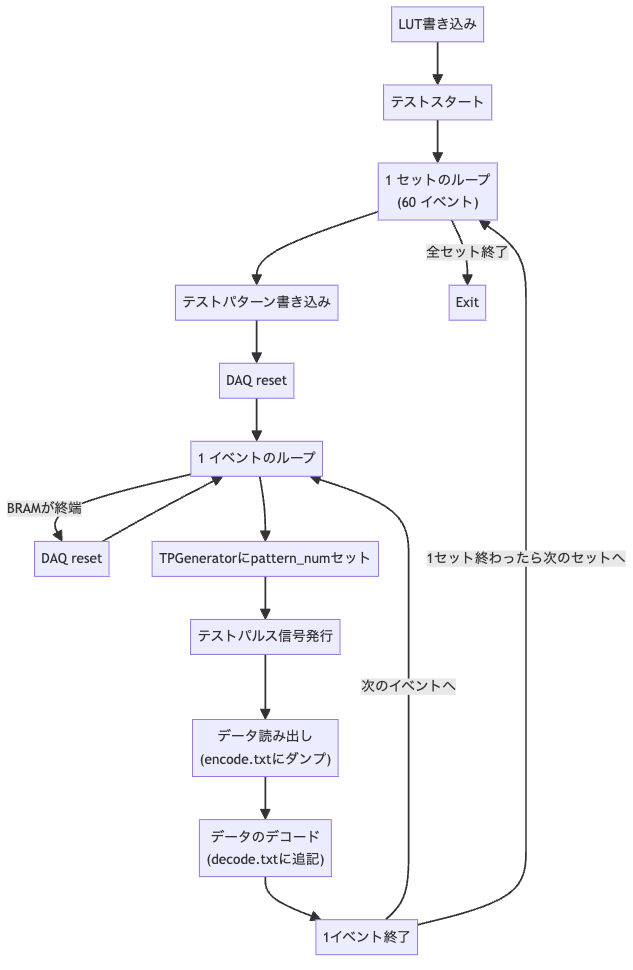
\includegraphics[width=10cm]{fig/Test/Flowchart.png}
\caption[アプケーションのフローチャート]{アプリケーションのフローチャート}
\label{Flowchart}
\end{figure}

試験の準備としてLUTの書き込みを行う。LUTに利用されているURAMはファームウェア上で初期値を設定することができないため、ファームウェアを焼き直すたびに書き込み直す必要がある。Wire Strip CoincidenceまでのすべてのLUTを書き込むのに概ね20分程度要する。

シミュレーションの実行はTest Pattern Generatorに一度に書き込めるイベント数である60イベントを1セットとして、テストパターンの書き込みと60回のテストパターンの発射を繰り返す。1イベントのシミュレーションループでは、最初にTest Pulse Generatorのパターンナンバーを指定し、60イベントの中から取り出すイベント番号を指定する。次にマニュアルでテストパルス信号を駆動し、トリガーロジックにデータを入力する。トリガーロジックの出力は読み出し回路を経てエンコードされたのち、MPSoC上のBRAMに格納される。格納されたデータをMPSoCのPSから取り出し、アプリケーション上でデコード作業を行う。デコードされたビット配列は最終出力としてSDカード上のテキストファイルにダンプされる。イベントのループを回している過程で、MPSoCのBRAMがfullになった場合はその都度リセットをかける。

\section{無限運動量飛跡を用いた試験}
\label{sec_IMT}

本章では無限運動量飛跡と呼ばれるトイデータセットを用いて行った、トリガー回路の初等的な試験について述べる。無限運動量飛跡とは、衝突点から直線的にTGC検出器に入射するミューオンをエミュレートした試験用のイベントであり、トリガーロジックとしては100 \%再構成できるべきイベントセットである。このイベントセットに対するTGC BW コインシデンスの応答を調べることで、実装したトリガーロジックが期待通り動作していることを確かめる。

以下ではまず先行研究で開発された無限運動量飛跡生成機構について述べた後、実機試験システムを用いた試験結果について述べる。

\subsection{無限運動量生成機構}
\label{subsec_IMT_generation}

\subsubsection{スタッガードID}
前章で述べたようにTGC検出器は位置分解能向上、データ量の削減を実現するため、スタッガリング構造を取っている。ステーション内の2層または3層のガスチェンバーは、各チャンネルのカバーする$\eta$領域がずれるよう設置されており、ステーション内のコインシデンスをとることにより、位置分解能を2、3倍に高めた代表点を算出する。また、M3の各代表点と同じ$\eta$に位置するM1、M2の代表点に同じ番号が割り振られるよう定義したものをスタッガードIDとよぶ。スタッガードIDは各ステーション内の代表点に通し番号的に振られている訳ではなく、M3の代表点を起点に、その$\eta$に一番近いチャンネルを選ぶようにして値を割り振っている。\footnote{TGC検出器が設計された当初は、各ステーションで$\eta$の位置分解能が均一になるようにワイヤーがバンドルされていたため、ステーション内で通し番号的にスタッガードIDを割り振ることができるはずだった。しかし、設置の段階でTGC検出器の設置位置がz方向にずれたため、これはできなくなった。}

% \begin{figure} 
% \centering
% 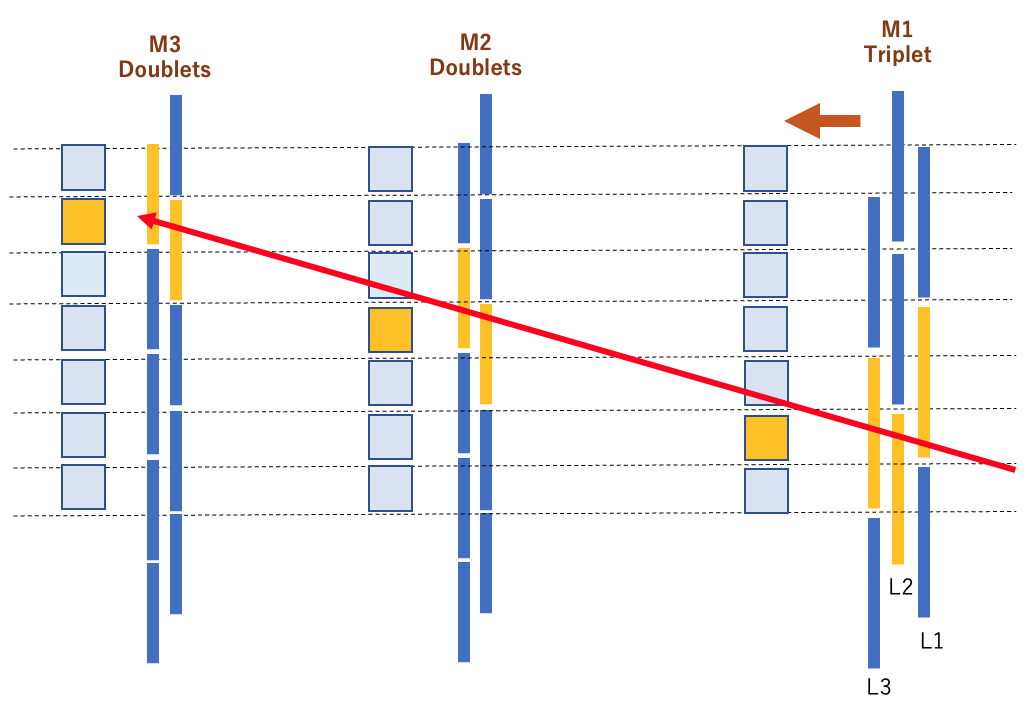
\includegraphics[width=16cm]{fig/Test/StaggerdID.png}
% \caption[スタッガードIDの概念図]{スタッガードIDの概念図}
% \label{StaggerdID}
% \end{figure}

スタッガードIDはケーブリングデータベースにより、各検出器のチャンネル番号と紐づけられている。テストパターン生成機構はそれを活用して、任意の代表点に入射する無限運動量飛跡を作成することができる。とある$\eta$位置に入射するミューオンをエミュレートしたテストパターンが作りたい場合、スタッガードIDを指定するだけで、それに対応する7層のヒット情報が一意に決められ、テストパターンが生成される。ストリップに対しても同様の仕掛けが作られており、$\eta$と$\phi$のスタッガードIDをそれぞれ指定することで、任意の ($\eta$、$\phi$) に入射するミューオンを模したテストパターンを作成することができる。


\subsection{無限運動量飛跡を用いたトリガーロジックの試験}
トリガーロジックおよびLUTに対する最初の試験として、図\ref{InfMomentum}に示すようにM3のWire、Stripで張られる全2次元格子点に対して無限運動量飛跡を用意した。Wire Segment Reconstruction、Strip Segment Reconstruction、Wire Strip Coincidenceのそれぞれにおいて、すべてのイベントがトリガーをパスすることを確認することで、TGCの全領域にわたってトリガーロジックが期待通りに動作していることを検証する。フォワード領域にはWireのスタッガードチャンネルが243 ch、Stripのスタッガードチャンネルが63 chあり、合計15,309の格子点が存在する。ECは$\phi$0、$\phi$1 それぞれでWireスタッガードチャンネル579 ch、Stripスタッガードチャンネル63 chで合計36,477の格子点が存在する。

\begin{figure} 
\centering
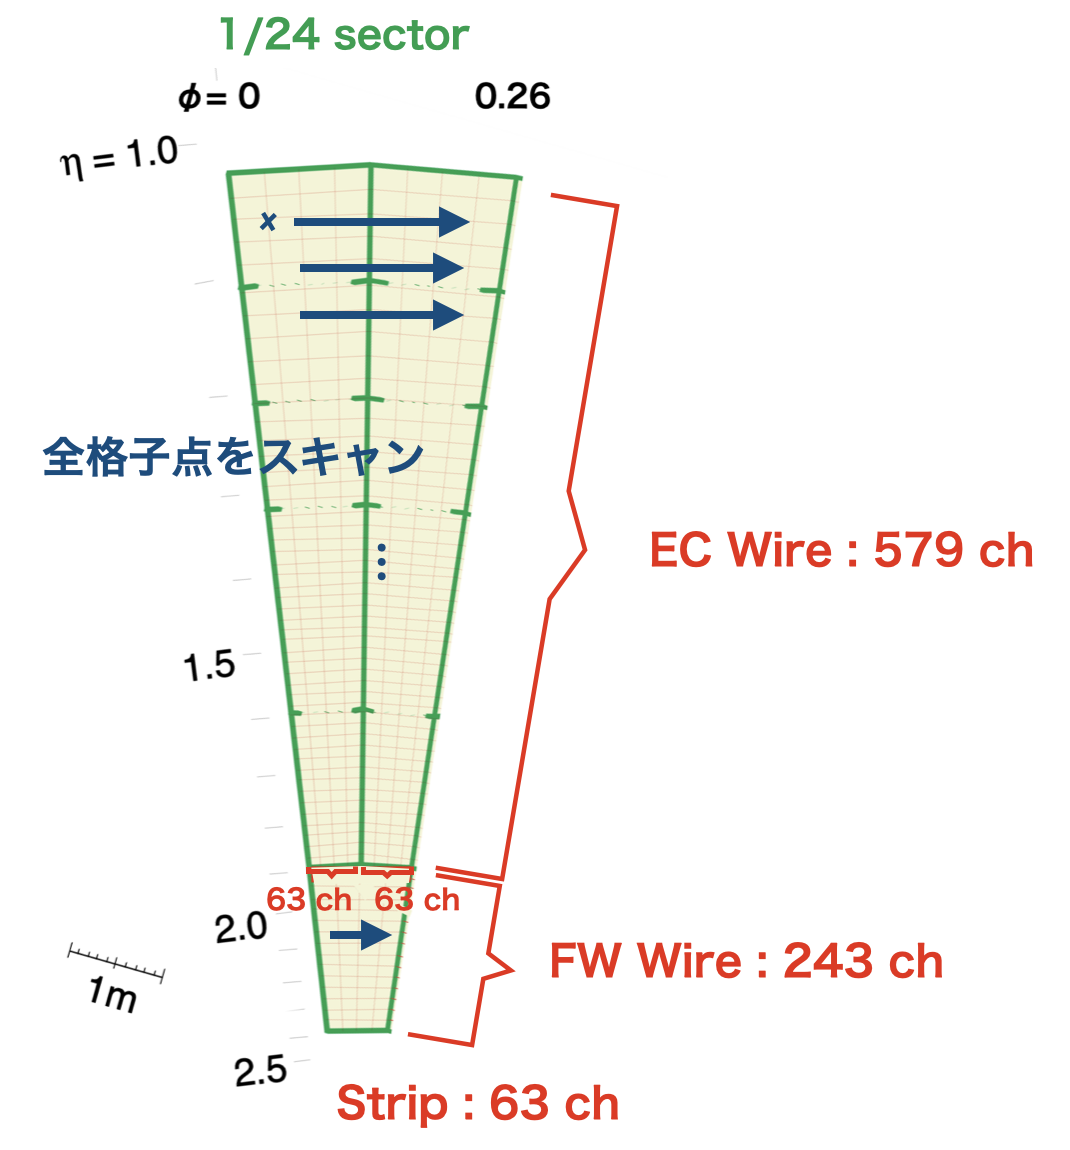
\includegraphics[width=10cm]{fig/Test/InfMomentum.png}
\caption[用意した無限運動量飛跡のデータセット]{用意した無限運動量飛跡のデータセット。FW、EC領域に存在する全2次元格子点に対して網羅的にテストパターンを用意。1枚のSLが担当するすべての領域でトリガーロジックが期待通り動作していることを調べる。}
\label{InfMomentum}
\end{figure}

図\ref{Inf_A_Strip}$\sim$図\ref{Inf_A_WS}に各モジュールごとの結果を示す。横軸にStripのスタッガードID、縦軸にWireのスタッガードIDをとり、飛跡再構成に失敗した格子点を黒で塗りつぶしている。飛跡再構成に成功したイベントの割合を表\ref{tab:InfMomentum}にまとめる。

\begin{figure}
\begin{minipage}[b]{.5\linewidth}
    \centering
    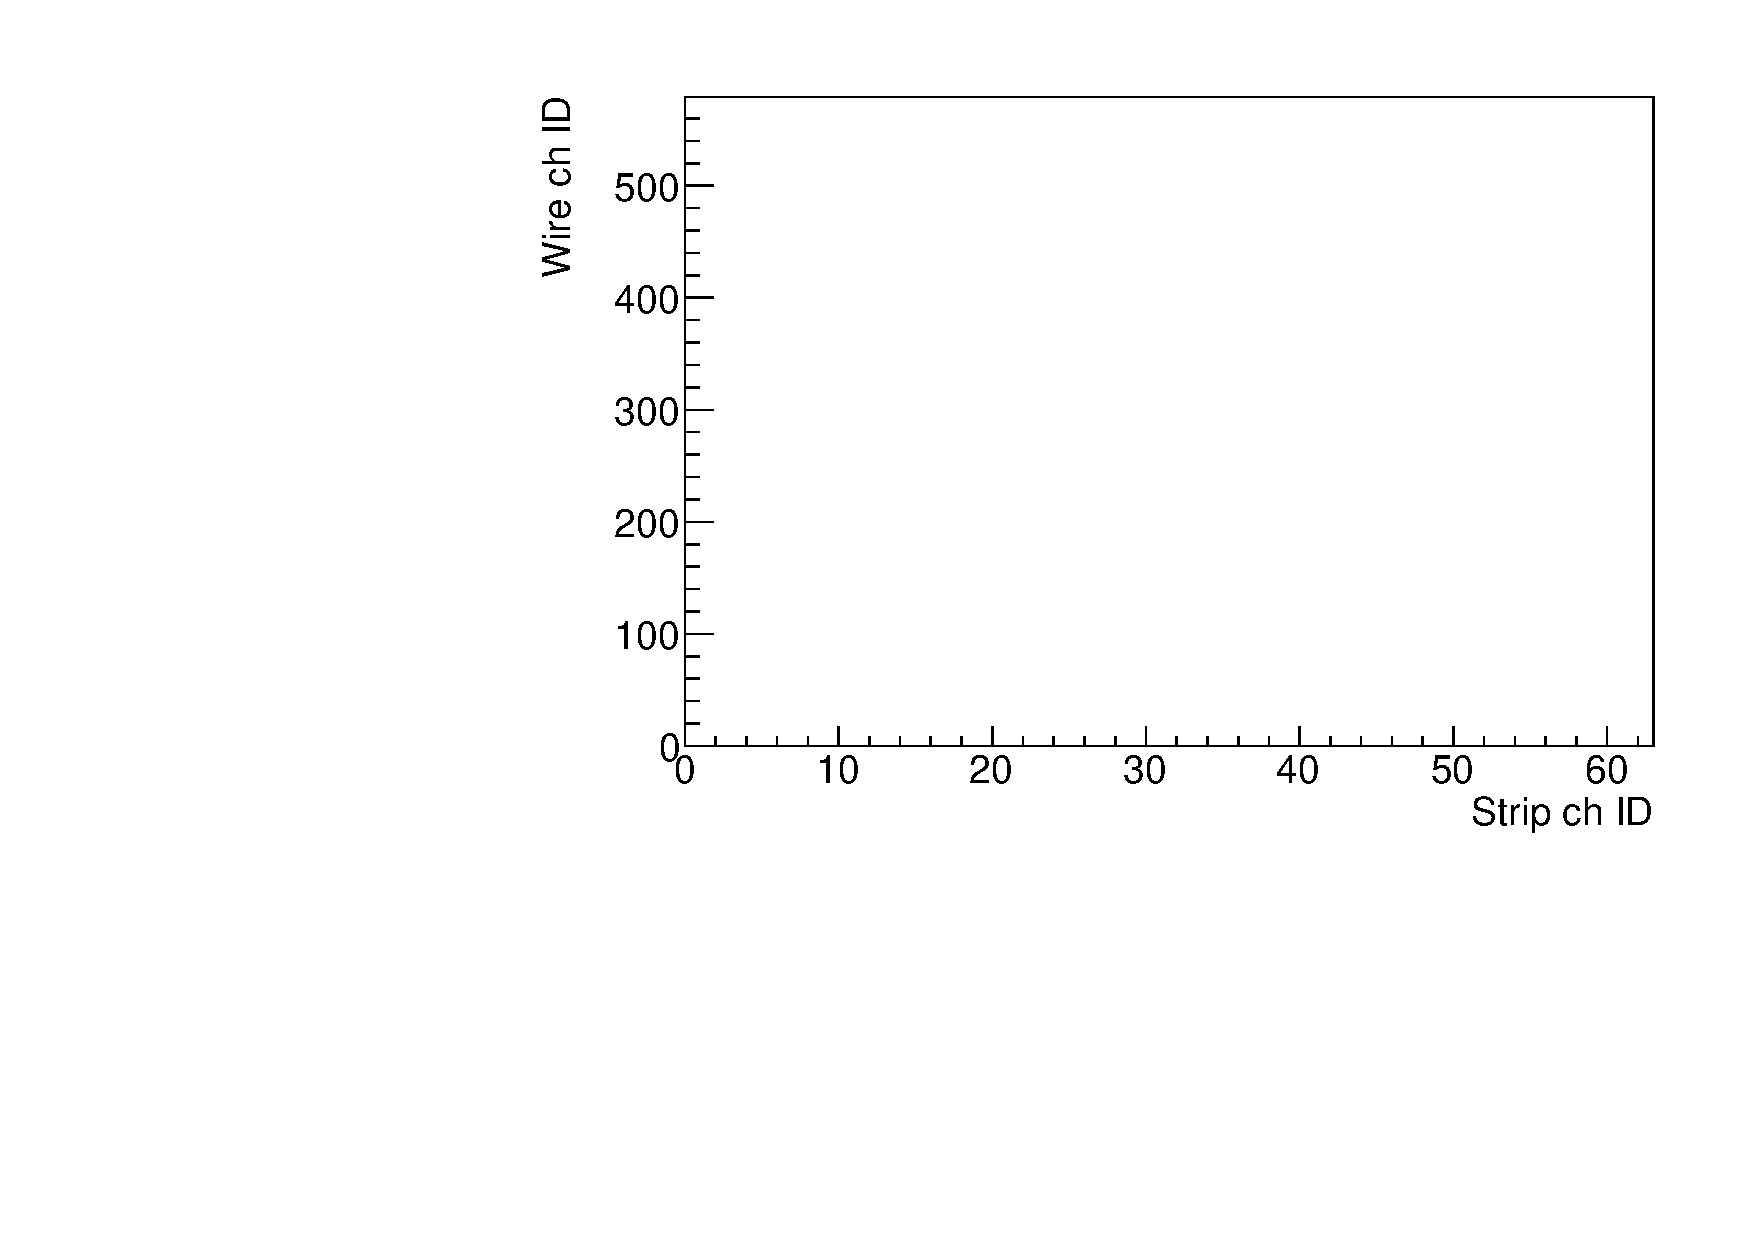
\includegraphics[height=6cm]{fig/Test/A_InfEC0_strip.pdf}
    \subcaption{エンドキャップ$\phi\,$0領域の結果}
\end{minipage}
\begin{minipage}[b]{.5\linewidth}
    \centering
    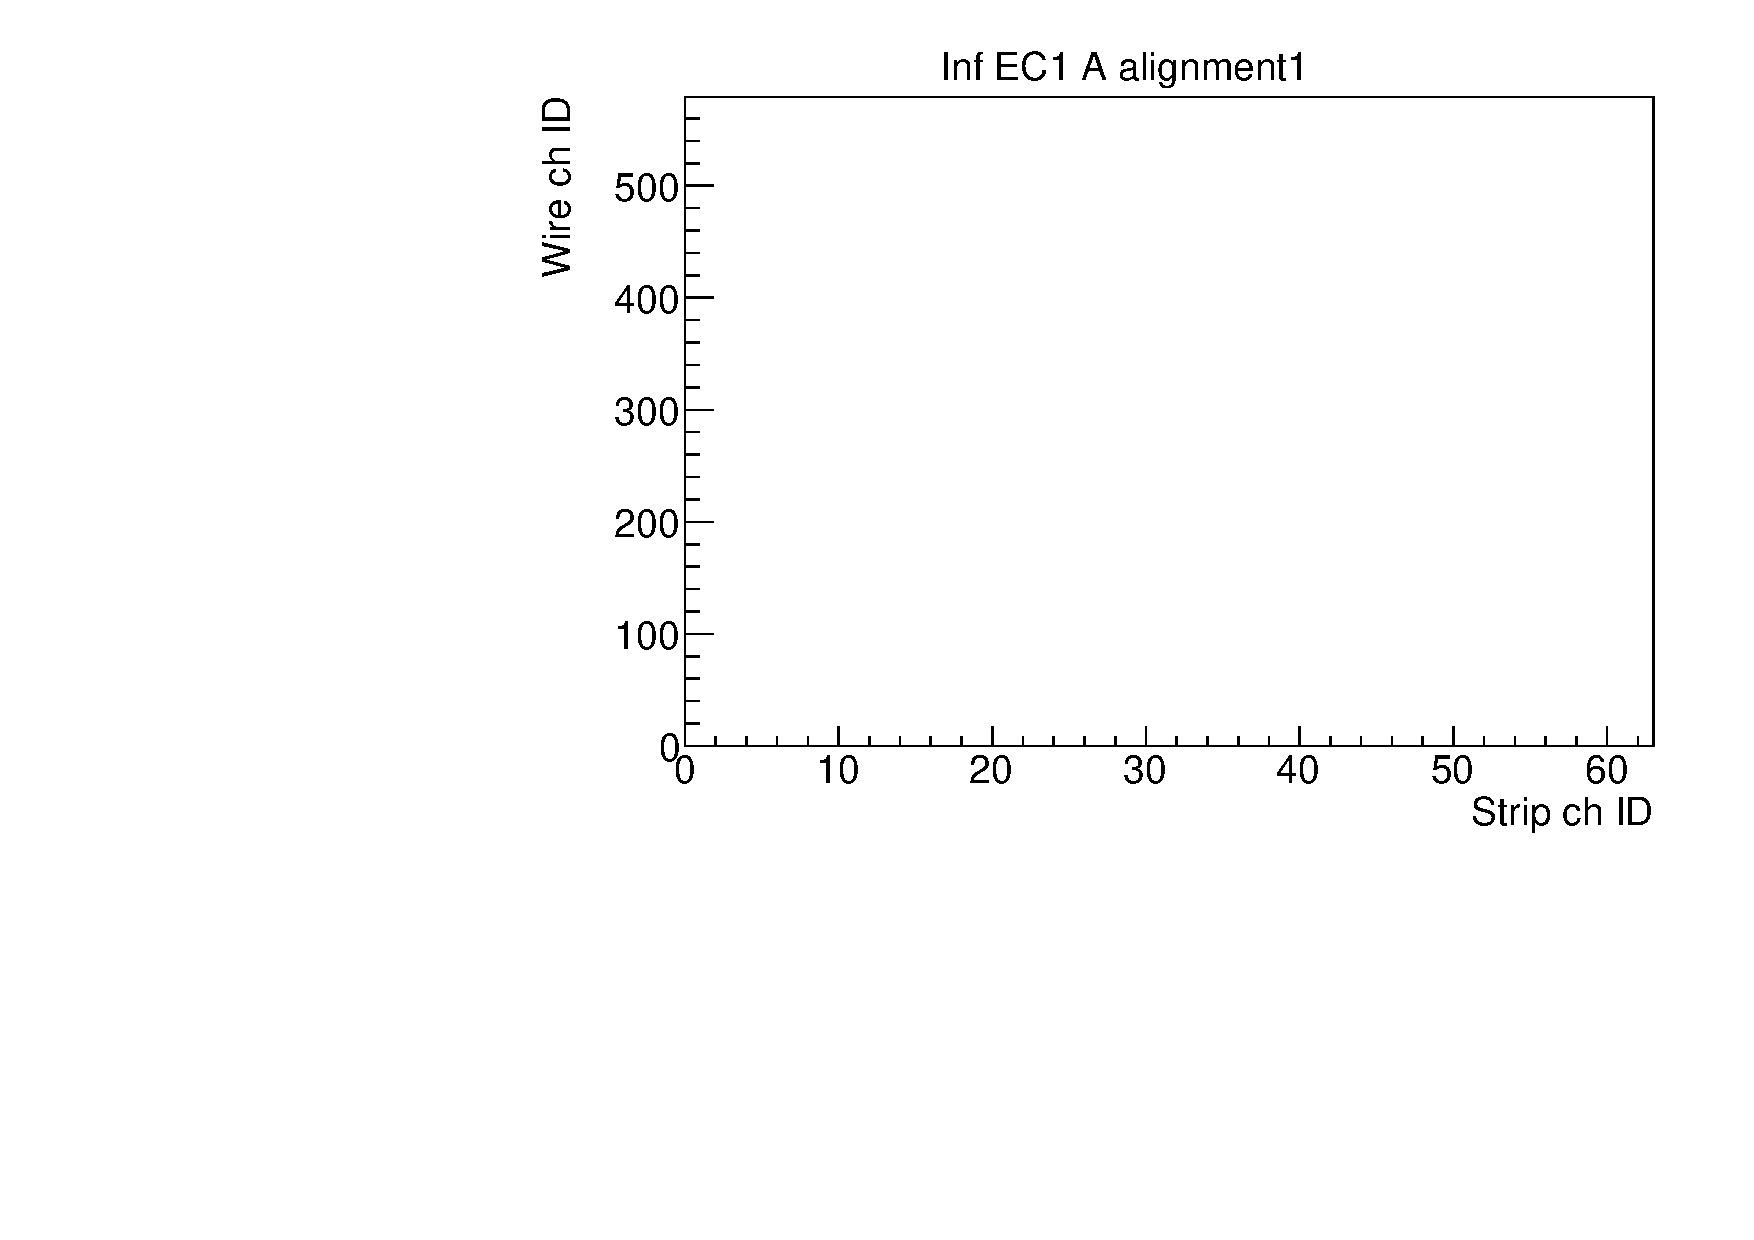
\includegraphics[height=6cm]{fig/Test/A_InfEC1_strip.pdf}
    \subcaption{エンドキャップ$\phi\,$1領域の結果}
\end{minipage}\\
\begin{minipage}[b]{\linewidth}
    \centering
    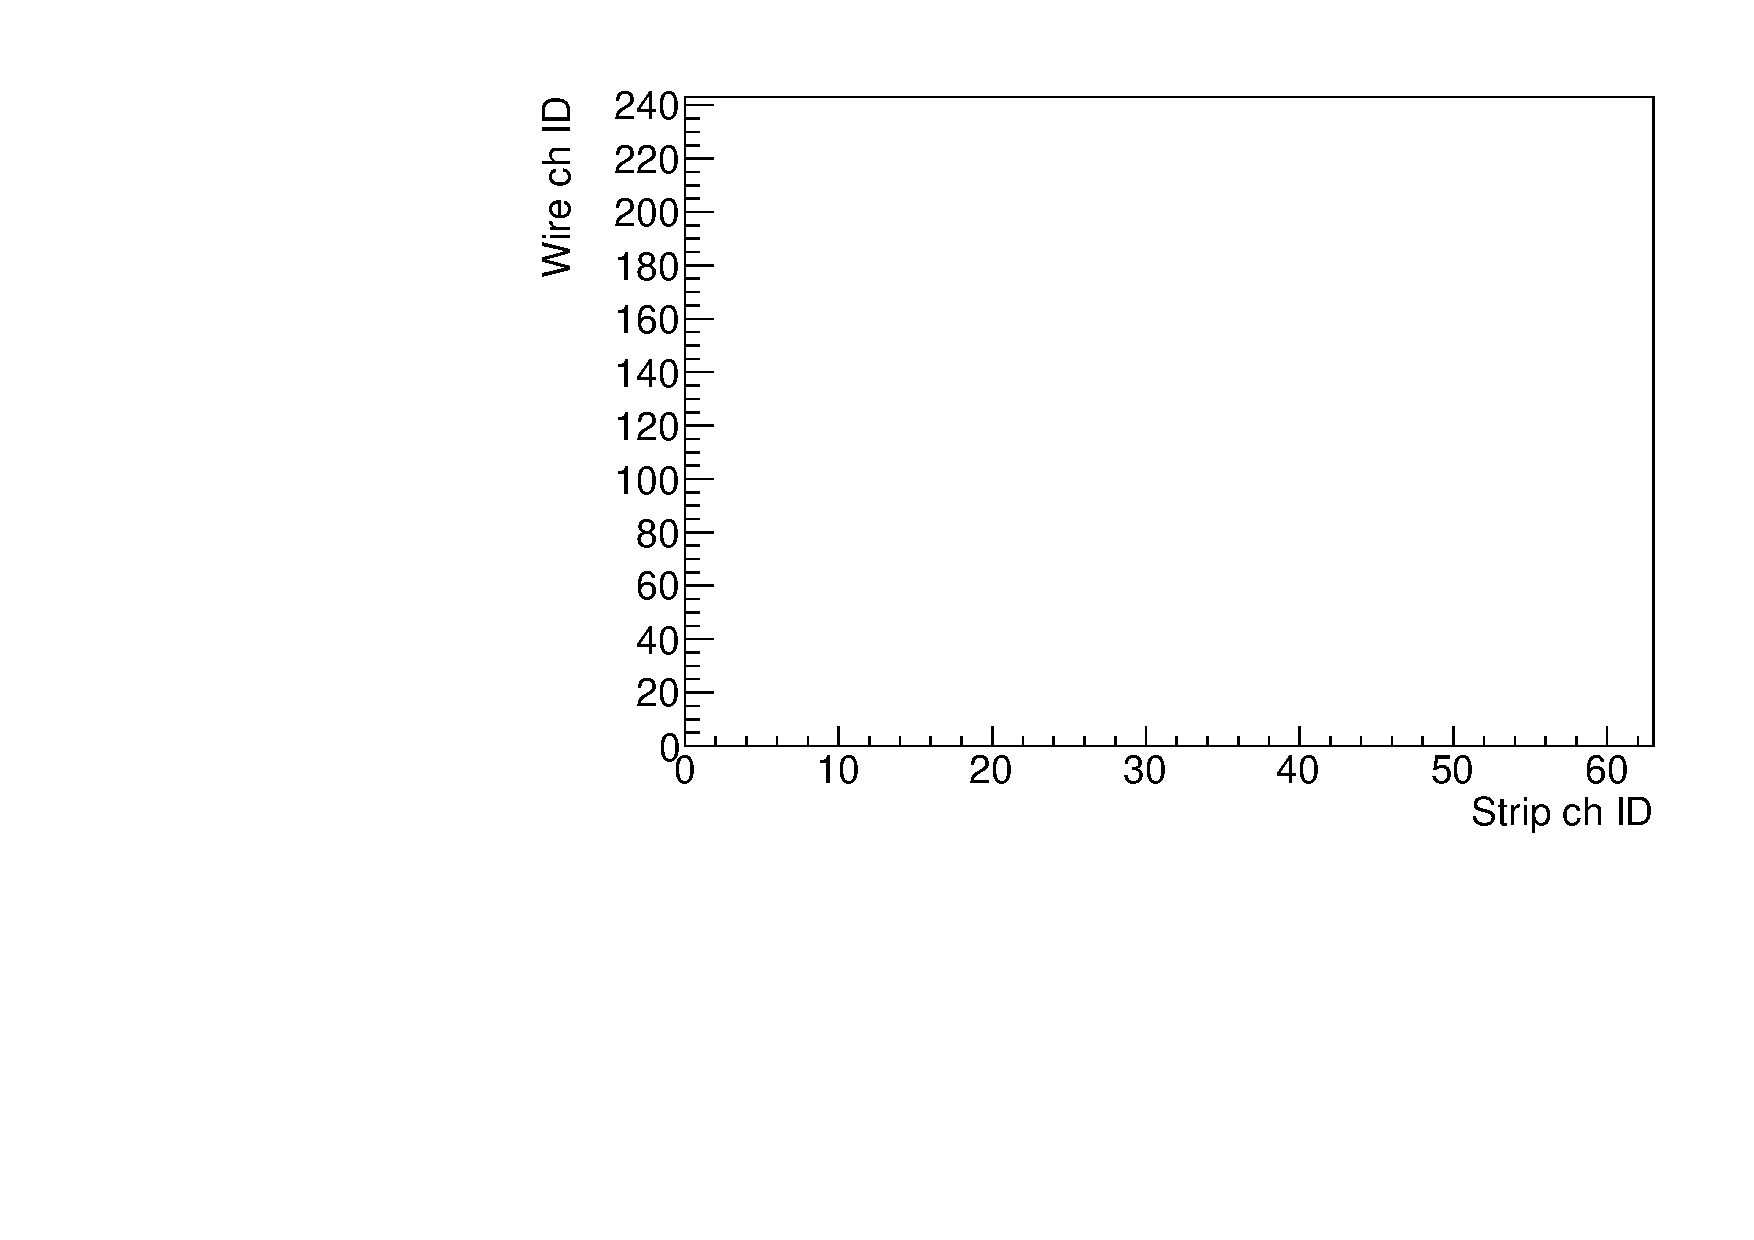
\includegraphics[height=6cm]{fig/Test/A_InfFW_strip.pdf}
    \subcaption{フォワード領域の結果}
\end{minipage}
\caption[異なる画像形式の比較]{無限運動量飛跡に対する、Strip Segment Reconstructionの応答。}
\label{Inf_A_Strip}
\end{figure}

\begin{figure}
    \begin{minipage}[b]{.5\linewidth}
        \centering
        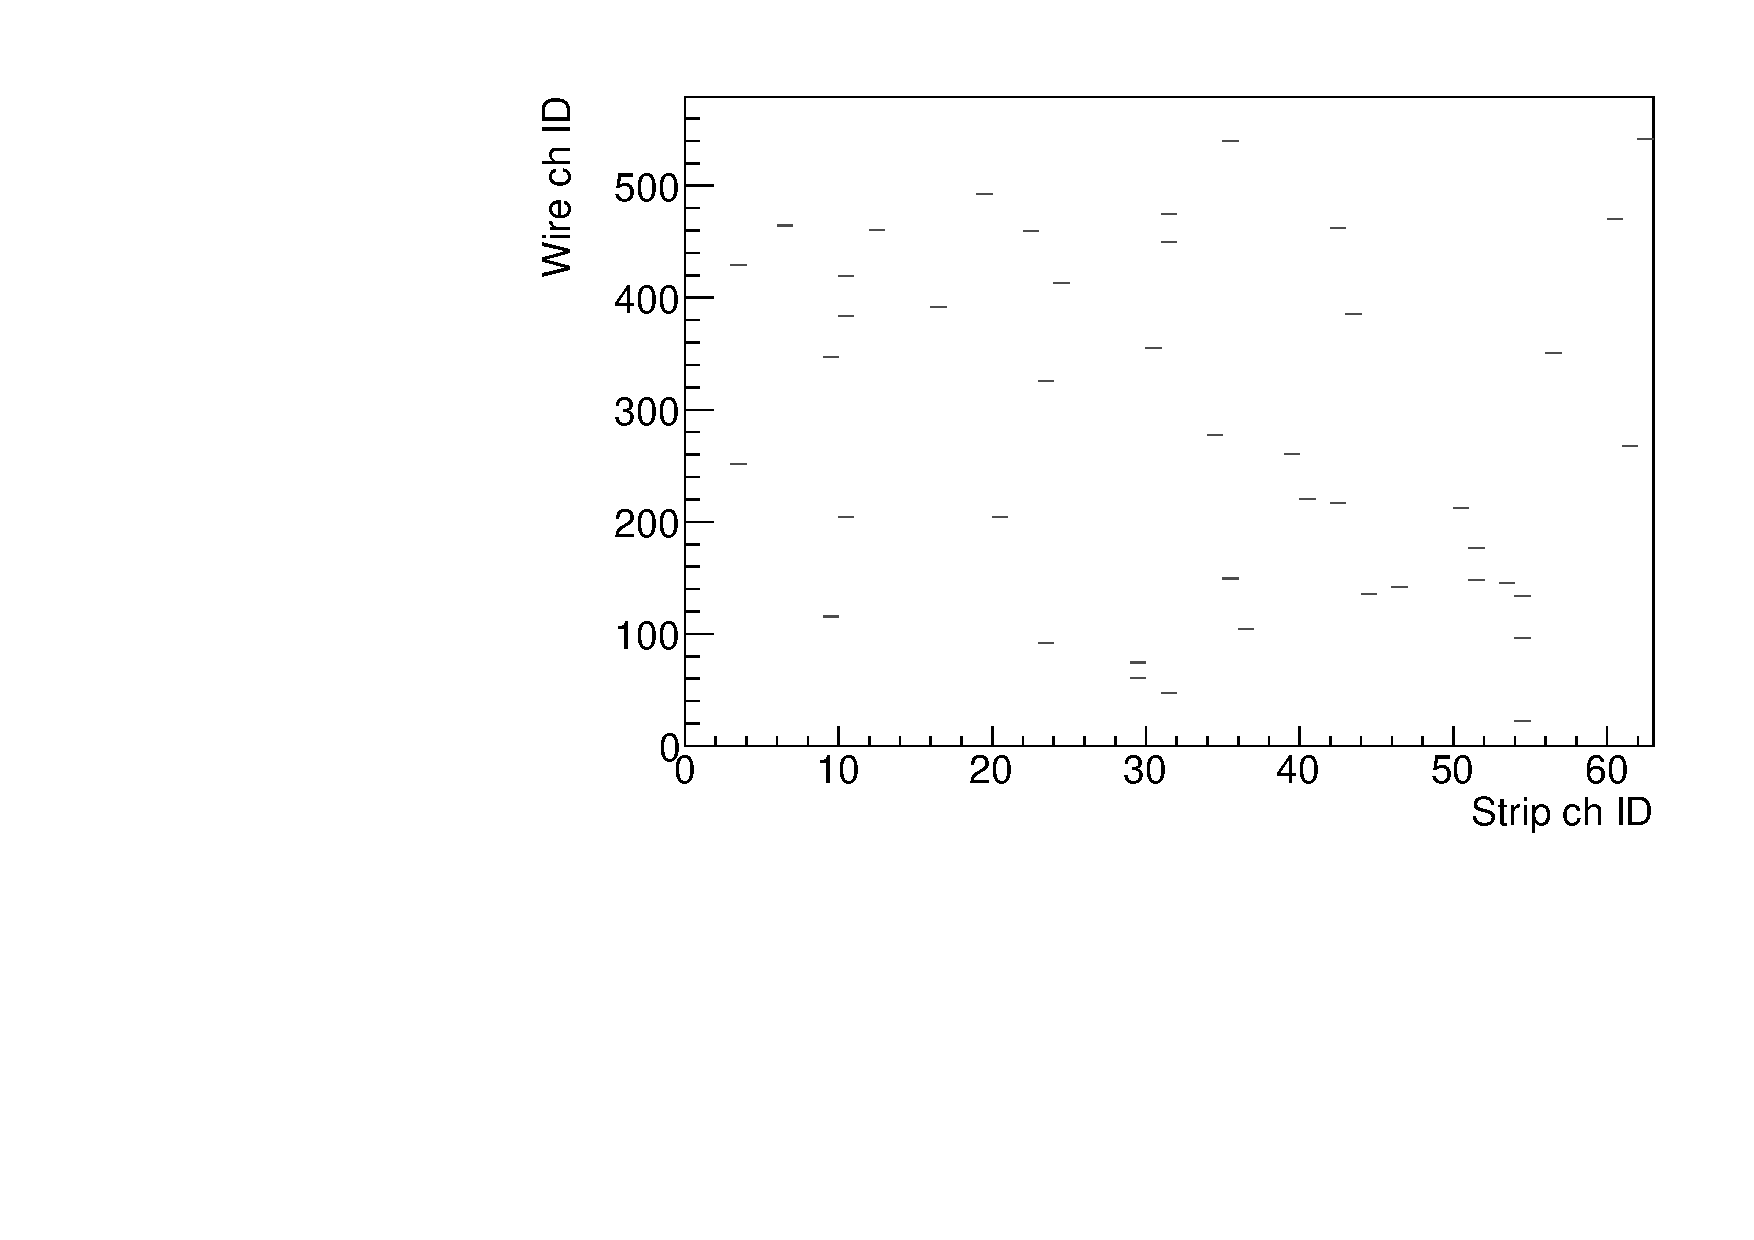
\includegraphics[height=6cm]{fig/Test/A_InfEC0_wire.pdf}
        \subcaption{エンドキャップ$\phi\,$0領域の結果}
    \end{minipage}
    \begin{minipage}[b]{.5\linewidth}
        \centering
        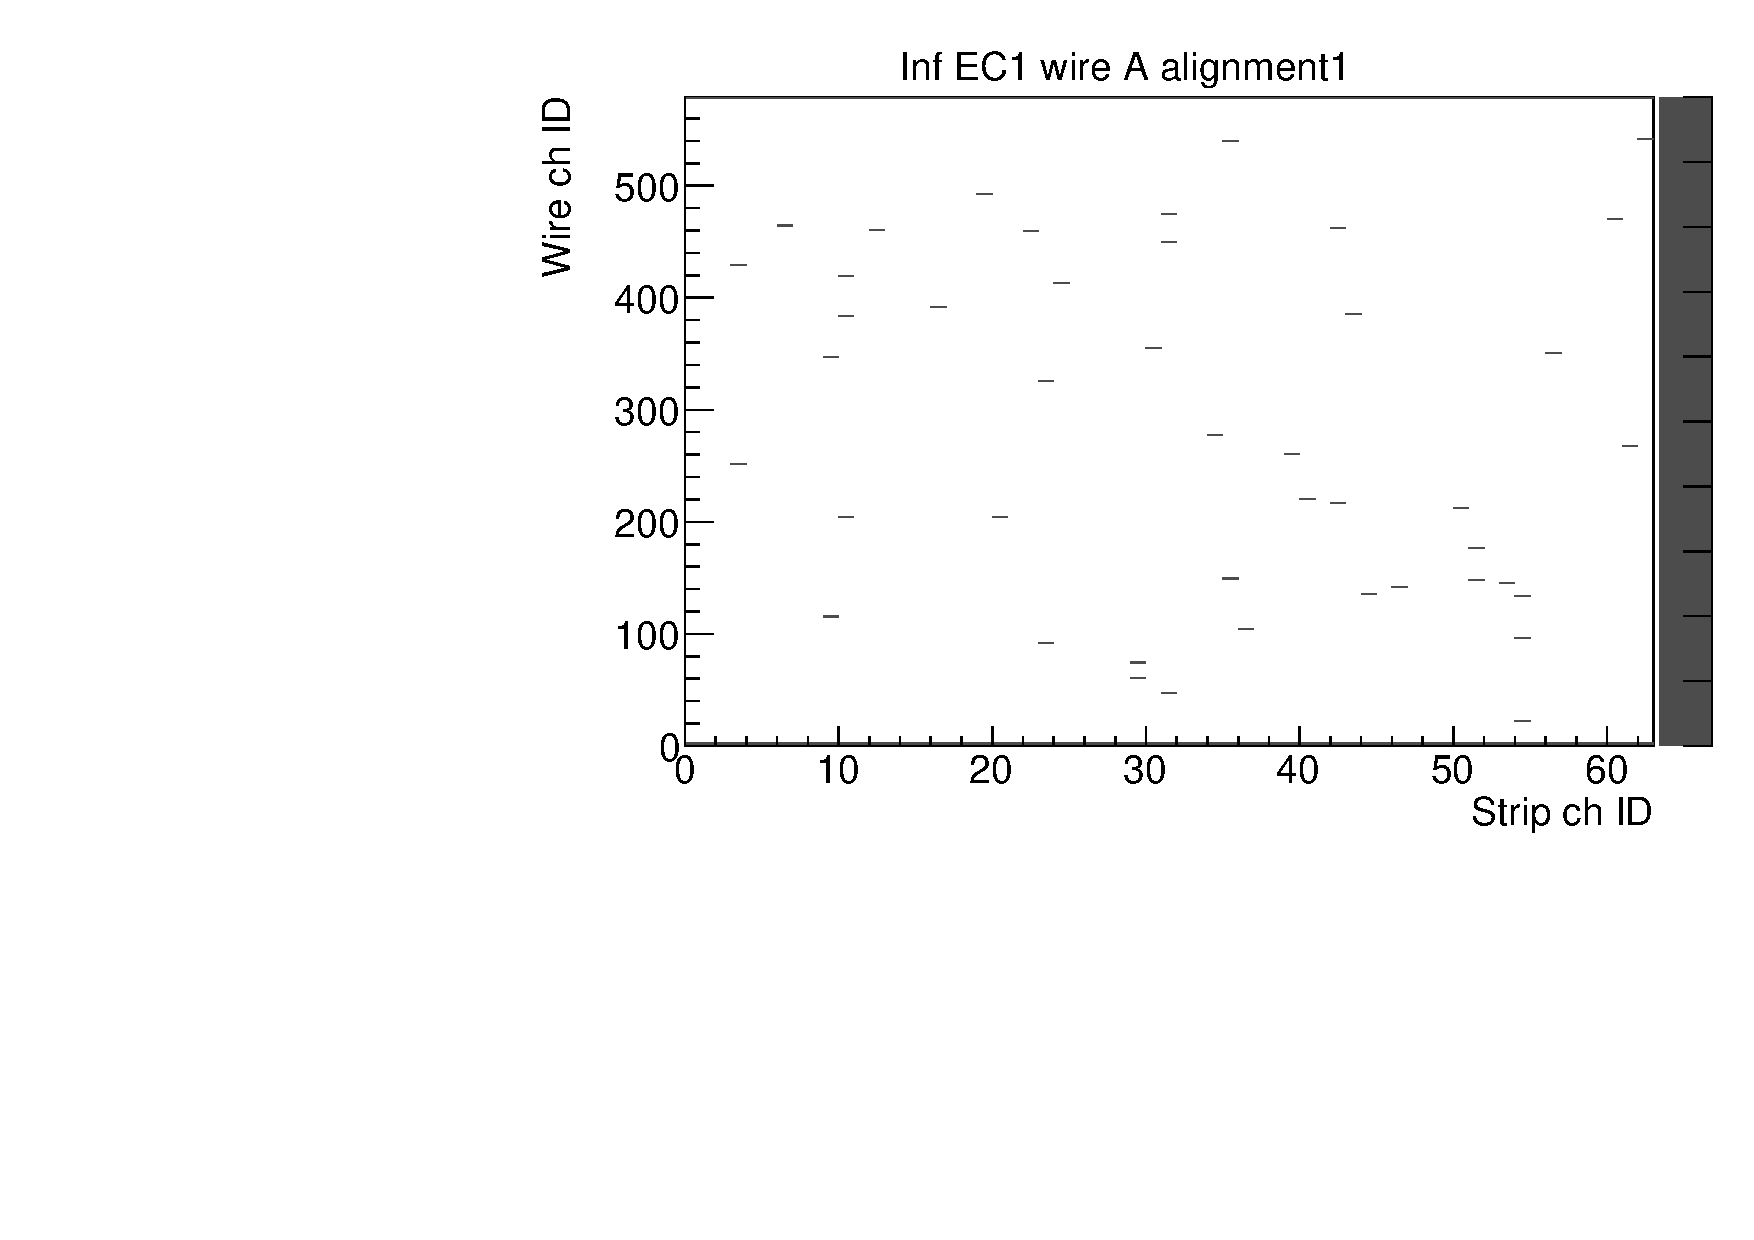
\includegraphics[height=6cm]{fig/Test/A_InfEC1_wire.pdf}
        \subcaption{エンドキャップ$\phi\,$1領域の結果}
    \end{minipage}\\
    \begin{minipage}[b]{\linewidth}
        \centering
        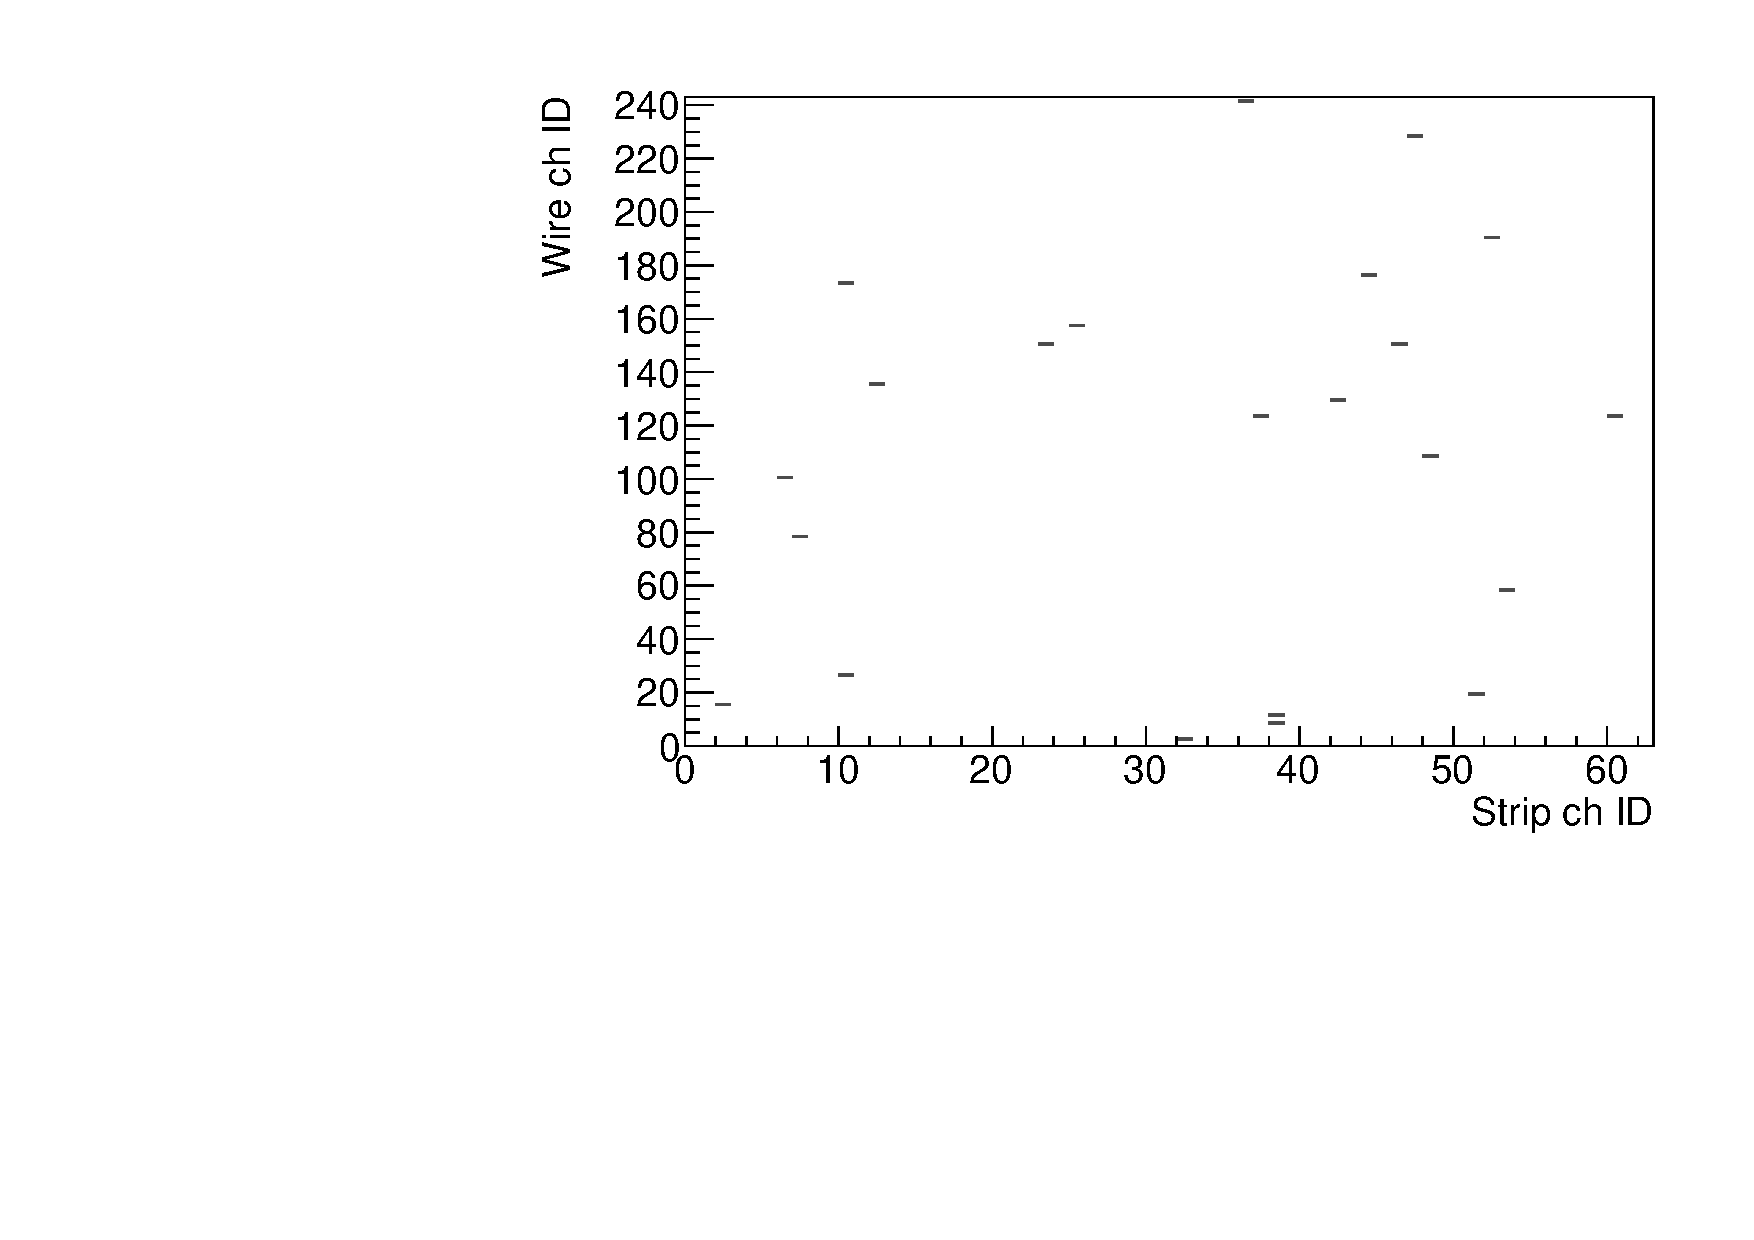
\includegraphics[height=6cm]{fig/Test/A_InfFW_wire.pdf}
        \subcaption{フォワード領域の結果}
    \end{minipage}
    \caption[異なる画像形式の比較]{無限運動量飛跡に対する、Wire Segment Reconstructionの応答。}
    \label{Inf_A_Wire}
\end{figure}

\begin{figure}
    \begin{minipage}[b]{.5\linewidth}
        \centering
        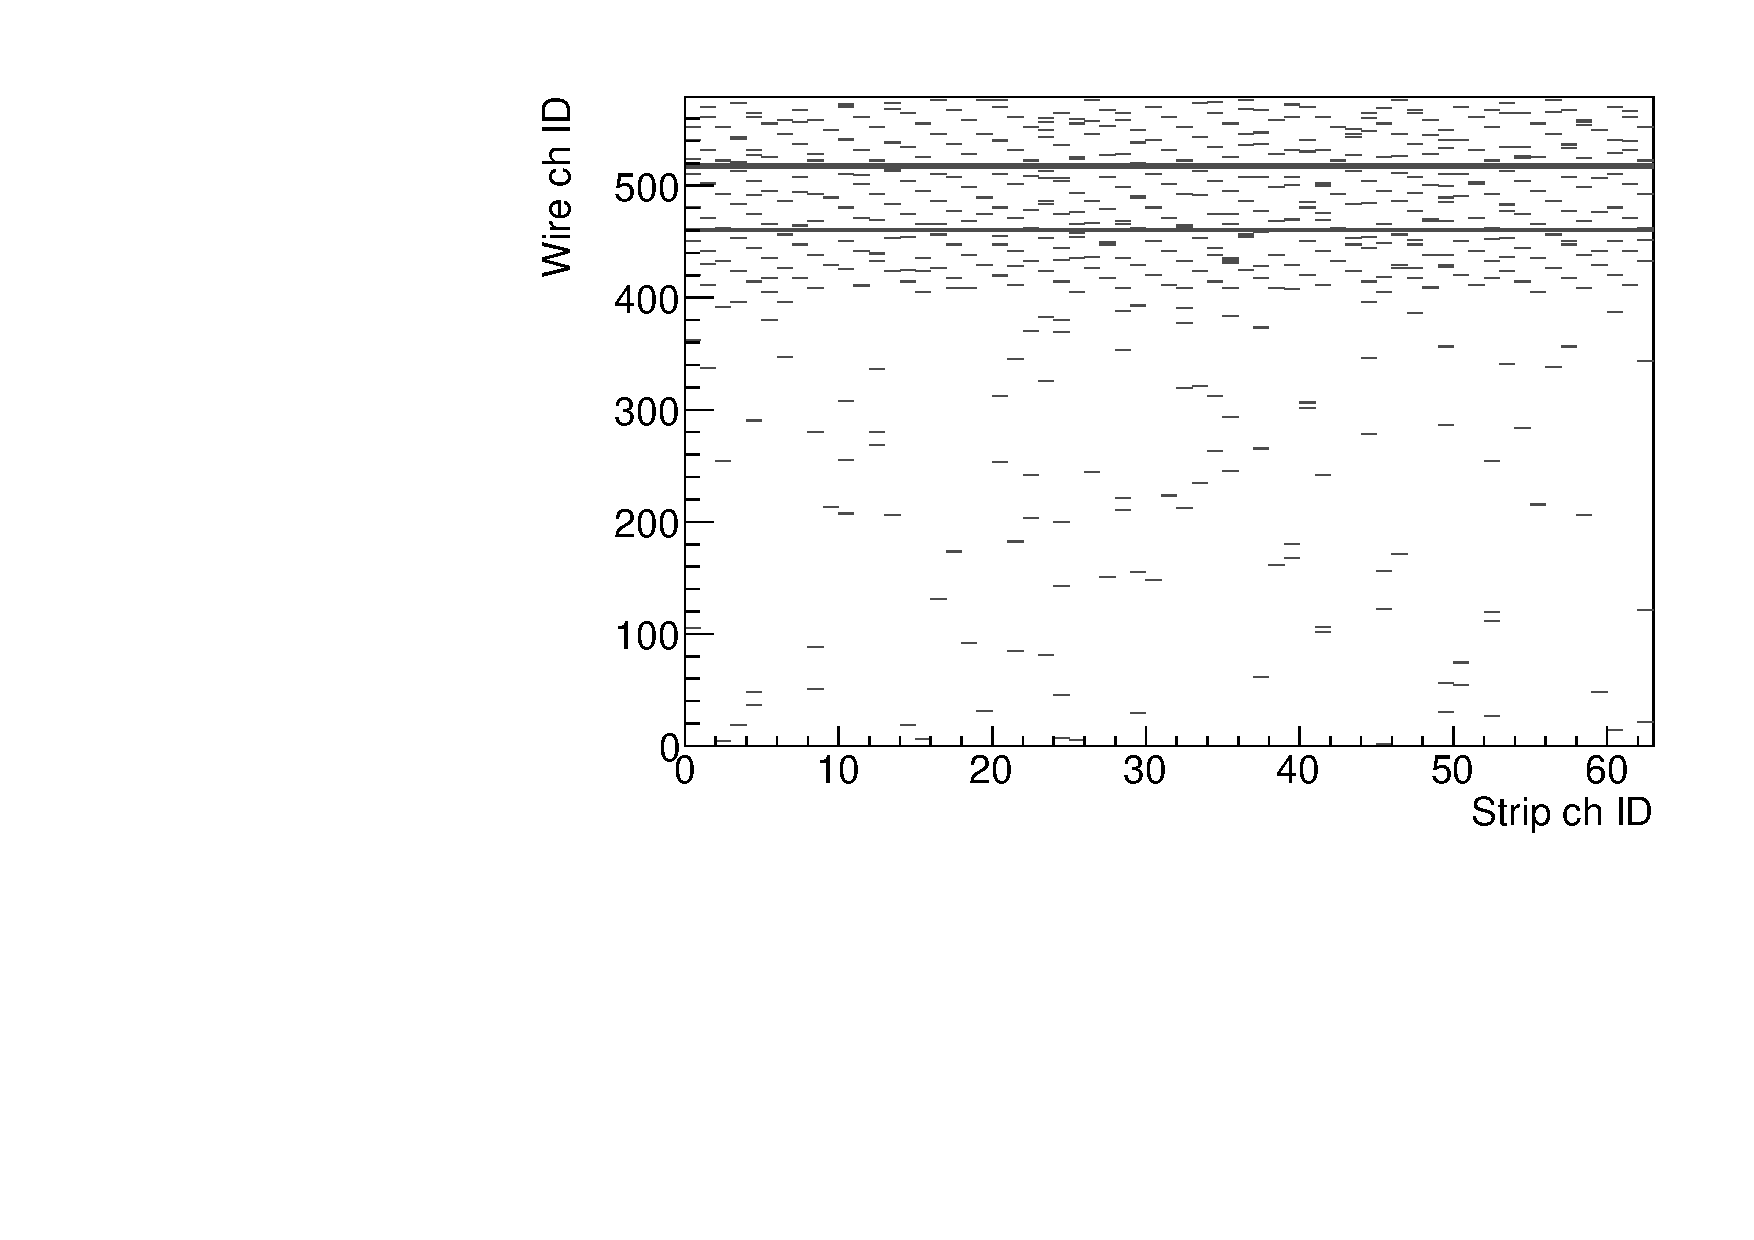
\includegraphics[height=6cm]{fig/Test/A_InfEC0_WS.pdf}
        \subcaption{エンドキャップ$\phi\,$0領域の結果}
    \end{minipage}
    \begin{minipage}[b]{.5\linewidth}
        \centering
        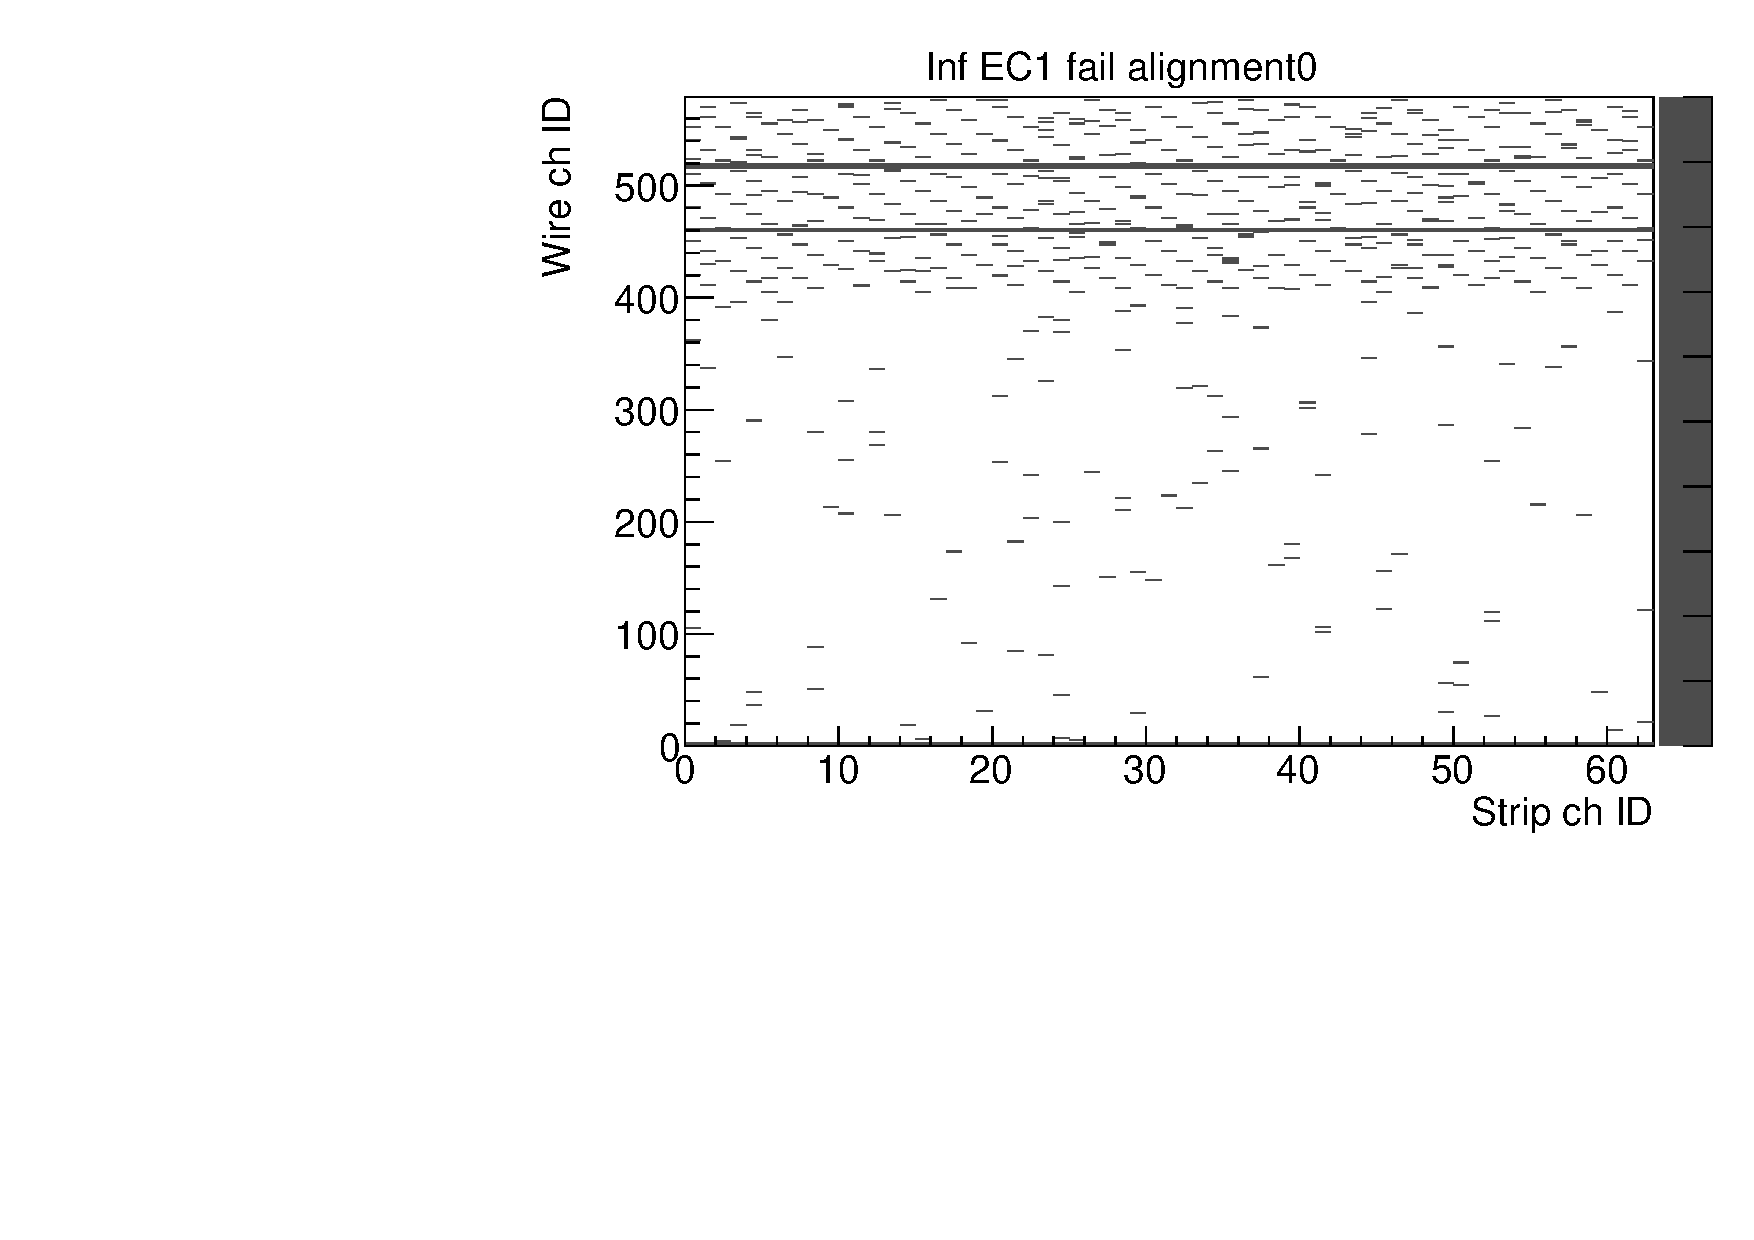
\includegraphics[height=6cm]{fig/Test/A_InfEC1_WS.pdf}
        \subcaption{エンドキャップ$\phi\,$1領域の結果}
    \end{minipage}\\
    \begin{minipage}[b]{\linewidth}
        \centering
        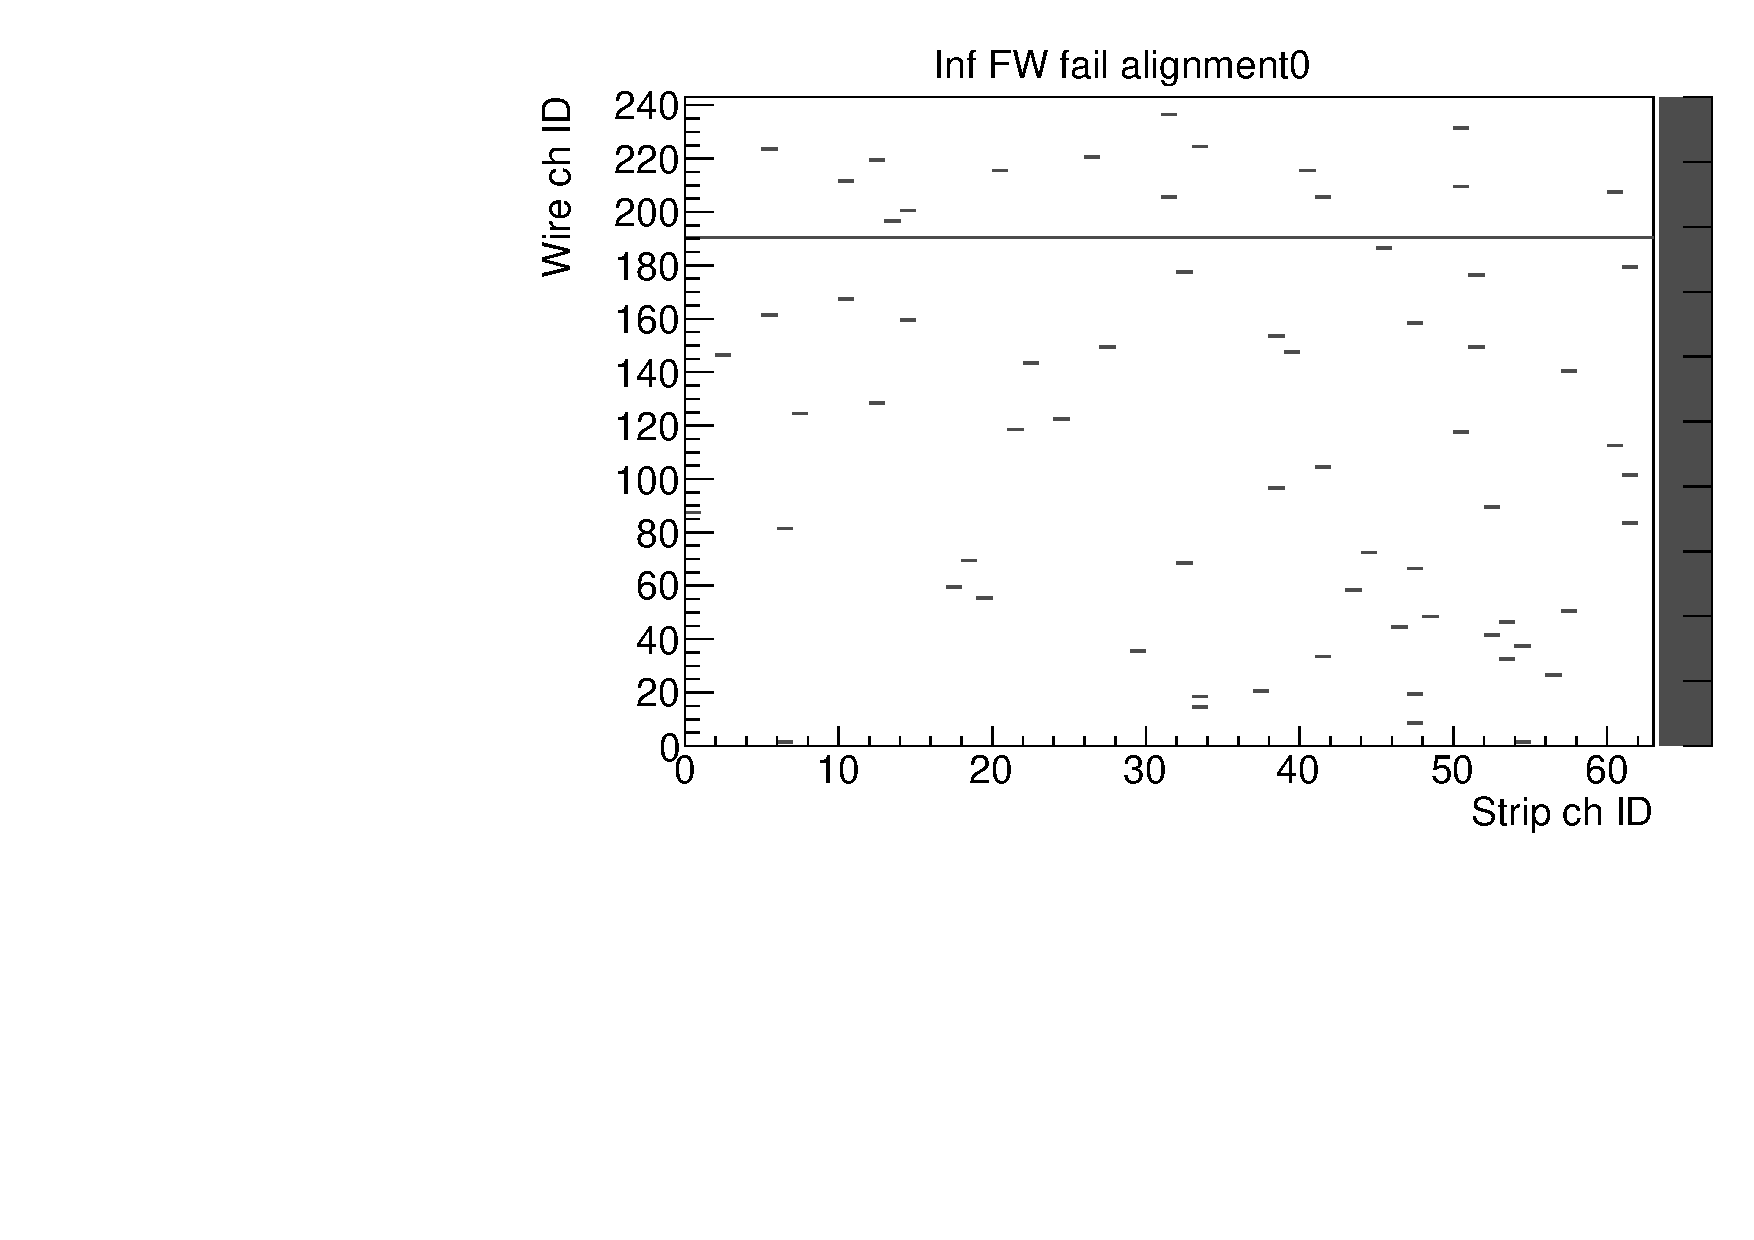
\includegraphics[height=6cm]{fig/Test/A_InfFW_WS.pdf}
        \subcaption{フォワード領域の結果}
    \end{minipage}
    \caption[異なる画像形式の比較]{無限運動量飛跡に対する、Wire Strip Coincidenceの応答。}
    \label{Inf_A_WS}
\end{figure}

\begin{table}[]
    \centering
    \caption[無限運動量飛跡に対するトリガーロジックの応答]{無限運動量飛跡に対する飛跡再構成の成功率}
    \label{tab:InfMomentum}
    \begin{tabular}{|c|c|c|c|}
    \hline
        & \begin{tabular}[c]{@{}c@{}}Strip Segment \\ Reconstruction\end{tabular} & \begin{tabular}[c]{@{}c@{}}Wire Segment\\ Reconstruction\end{tabular} & \begin{tabular}[c]{@{}c@{}}Wire Strip \\ Coincidence\end{tabular} \\ \hline\hline
    FW  & 100 \%                                                                  & 99.9 \%                                                               & 99.2 \%                                                           \\ \hline
    EC0 & 100 \%                                                                  & 99.7 \%                                                               & 97.0 \%                                                           \\ \hline
    EC1 & 100 \%                                                                  & 99.9 \%                                                               & 96.5 \%                                                           \\ \hline
    \end{tabular}
\end{table}

\paragraph{Strip Segment Reconstruction}  
\par 
Strip Segment Reconstructionではフォワード領域とエンドキャップ領域の全領域で飛跡再構成に成功した。この結果はChannel Mapping、Strip Station Coincidence、Strip Segment Reconstruction、のHDL実装がミスなく行われたこと、作成されたLUTが抜けなく実装されていること、そしてLUTの書き込みパスなどトリガーを稼働させるのに必要なコントロール機能が正確に動作していることを示している。さらに、この結果は実機試験システム自体が正確に動作していることも示唆している。MPSoCからのテストパターンを書き込むパスとトリガーロジックの読み出しパスは安定して動作しており、TTC emulator、トリガーロジック、読み出しパスが固定レイテンシーで制御されていることが保証される。これらのコントロールおよび読み出しパスは実験本番でも使われるシステムであり、SL統合ファームウェア全体が精度良く動作していることを示すしている。この結果を得られるまでの過程でStrip LUTのミスを発見し、修正を行った。デバッグの過程はAppendix\ref{sec:appendix:infinite-momentum-tracks}に詳述する

\paragraph{Wire Segment Reconstruction}  
\par
Wire Segment Reconstructionでは、フォワード領域で99.9 \% ( 15,287 / 15,309 )、エンドキャップ$\phi\,$0領域で99.7 \%(35,370 / 36,477)、エンドキャップ$\phi\,$1領域で99.9 ( 36.181 / 36.477 )の飛跡再構成に成功した。しかし、エンドキャップ$\phi\,$1領域のはWire スタッガード ID $0 \sim 2$ の範囲では、全てのイベントで飛跡再構成に失敗している。また、全領域においてで特定の構造を持たない$\mathcal{O}(0.1\,\%)$のInefficiencyが観測された。

前者のInefficiencyに関しては、Bitwiseシミュレーターでも確認されており、これはTGC検出器の特性によるものであると理解されている。$\phi1$領域の$\eta\sim$2.0付近の領域ではM3がM1よりも広い$\eta$範囲をカバーしているため、M3をピボットとして無限運動量飛跡を作成すると、M1では担当するチャンネルが存在せず、コインシデンスが取れない。

後者のInefficiencyについては、Bitwiseシミュレーターでは確認されていないため、実機試験システムに固有の問題であると考えられる。調査により、飛跡再構成に失敗する格子点の位置には、データの取り直しに対して再現性がないことが明らかになった。失敗するイベントの割合は試験ごとに概ね一定で、Wireでは約0.1 \%である。現状、この問題がハードウェア上のトリガー回路自体の問題に起因するのか、あるいは読み出し回路の問題に起因するのかの区別がついておらず、問題の解決には至っていない\footnote{トリガー読み出し回路はモジュールごとに独立した回路になっており、読み出すデータの出力ビット幅の違いにより、Ineffficiencyが見れたり見られなかったりする可能性は排除できない}。次節以降の試験でもこのInefficiencyは存在すると考えられるが、本論文で議論するInefficiencyは $\mathcal{O}(10 \%)$ 程度のものであるため、このInefficiencyは実機システムに付随する避けられないものとして受け入れ、議論をすすめる。

この結果を得られるまでの過程で無限運動量飛跡生成機構に問題を発見し、修正を行った。デバッグの過程はAppendix\ref{sec:appendix:infinite-momentum-tracks}に詳述する。


\paragraph{Wire Strip Coincidence}  
\par
Wire Strip Coincidence では、フォワード領域で 99.6 \% ( 15,179 / 15,309 ) 、エンドキャップ$\phi\,$0領域で 97.0 \%(35,390 / 36,477) 、エンドキャップ$\phi\,$1領域で 96.5 ( 35.201 / 36.477 ) の飛跡再構成に成功した。フォワード領域ではWire スタッガードID 190 番に該当する飛跡が全て再構成されないことが確認された。エンドキャップ領域では、Wire スタッガード ID 410 番以降の領域で、$\phi0$と$\phi1$のどちらにも規則的な構造を持ったInefficiencyが観測された。このInefficiencyは、同様のLUTを利用しているBitwiseシミュレーターでは再現されないため、LUTの原因ではなくHDLの問題であると考えられる。Wire Strip Coincidence ではWire スタッガード IDが419より小さい領域は32 regionで処理され、大きい領域は8 regionで処理される。このため、構造的なInefficiencyは8 regionのファームウェアのバグである可能性が高い。今後VivadoシミュレーターとBitwiseシミュレーターの途中出力を比較し、バグが発生じている箇所を特定し、HDLの修正を進める予定である。

この試験により、TGC BW Coincidence の 95 \% 以上の領域でトリガーロジックが正常に動作していることが確認できた。一方で、トリガーロジックのHDL実装中に発生したと思われる不具合も発見できた。このような数 \% の局所的なInefficiencyは、網羅的かつ詳細なイベントセットを利用した検証だからこそ見つけられたもので、従来のVivadoシミュレーターでは見つけることが困難な問題であった。任意の位置に入射するミューオン飛跡をエミュレートできる無限運動量飛跡生成機構と、ハードウェア上で実際に動作するトリガー回路を大統計量で試験できる実機システムの真価が発揮された例である。実験開始前にこれらの誤りを発見し、修正することは最大パフォーマンスのミューオントリガーを実現する上で非常に重要である。


\section{モンテカルロデータを用いた性能評価}
\label{sec_SingleMuon}

本節ではより現実的なミューオンイベントに対するトリガー応答を調べるために行った、シングルミューオンモンテカルロデータを用いた試験について述べる。シングルミューオンとは、衝突点から検出器に1本のミューオンが入射する物理イベントをエミュレートしたデータセットである。このデータセットは、ミューオンがTGC検出器を素通りする事象、多重散乱により飛跡が曲げられる事象、制動放射や電磁シャワーによって複数のヒットが発生する事象など、実際に起こりうる物理過程を考慮したものになっている。したがって、より現実的なトリガー性能の評価が可能である。用意したデータセットの概要を表\ref{tab:SingleMuon}にまとめる。本試験ではトリガー回路自体の性能に焦点を当てた検証を行うため、TGC検出器のカバー範囲外のミューオンイベントは除外している。具体的にはテストパターン作成段階で、M1、M2、M3の各ステーションに少なくても1つのヒットがあることを要求している。

\begin{table}[]
    \centering
    \caption[用意したシングルミューオンモンテカルロデータの概要]{用意したシングルミューオンモンテカルロデータの概要}
    \label{tab:SingleMuon}
    \begin{tabular}{|c|c|}
    \hline
    Parameter        &                                                                                              \\ \hline
    $p_{\mathrm{T}}$ & $ 0 \, < \, p_{\mathrm{T}}\, < 50$ GeV flat                                                  \\ \hline
    $\eta$           & 1.06 \textless |$\eta$| \textless 2.4 flat                                                   \\ \hline
    $\phi$           & 0 \textless{} $\phi$ \textless 2\textbackslash{}pi flat                                      \\ \hline
    イベント数            & 500,000                                                                                      \\ \hline
    イベントカット          & \begin{tabular}[c]{@{}c@{}}1つのトリガーセクター内のM1、M2、M3各ステーションに\\ それぞれ1つ以上のヒットがあることを要求\end{tabular} \\ \hline
    \end{tabular}
\end{table}

\subsection{モジュールごとのEfficiency}
\par
\subsubsection*{Strip Segment Reconstruction}
この試験では \pt  が十分に大きい事象に対するトリガー応答を確認することを目的とし、Truth \pt  20 GeV 以上のミューオンイベントに対する検出効率を評価する。Efficiencyは式\ref{eq:Strip_Efficiency}のように定義する。

\begin{equation}
    \mathrm {Efficiency} = \frac{\mathrm{Strip\,Segment \,Reconstruction\,で\Delta\phi\,を再構成できたイベント数}}{\mathrm{Truth\,pt \,20 \,GeV以上のイベント数}}
    \label{eq:Strip_Efficiency}
\end{equation}

Strip Segment Reconstructionの検出効率の$\eta$および$\phi$依存性を図\ref{SM_A_strip}に示す。黒色の点はSL実機システムの出力結果、赤色の点はBitwise シミュレーターの出力結果を表している。$\phi$全領域での平均のトリガー検出効率は 97.4 \%であり、先行研究のソフトウェアシミュレーションの結果と矛盾のない結果が得られた。

トリガー効率の$\phi$依存性を見ると、チェンバーとチェンバーの境界に位置する領域 (エンドキャップ領域ではTGC BW 1周を48のトリガーセクターで分割するので 2$\pi$ / 48 = 0.26 おきにチェンバーの境界が存在) でEfficiencyが15 \%程度下がる傾向が確認された。事前の3つのステーションにヒットがあることを要求しているため、原理的にはチェンバー境界であってもEfficiencyが低下することはないはずであり、この点は改善が必要である。このInefficiencyはBitwiseシミュレーターでも再現されていることから、ファームウェアに固有の問題ではなく、共通に使用しているLUTや元のデータセットの不具合に起因するものであると考えられる。今後、Bitwiseシミュレーターを用いてイベントごとに飛跡再構成が失敗した理由を調査し、修正を進める。

また、Strip Segment Reconstructionでは実機とBitwiseシミュレーターの結果が概ね一致していることがわかった。これはBitwiseシミュレーターがHDLのロジックを極めて正確に再現できていることを示している。しかし、2 < $\eta$のFW領域、特に$\phi$チェンバー境界領域で、両者の出力に局所的な違いが生じている。原理的にはこの2つの出力は完全に一致するべきものであり、この差異はBitwiseシミュレーターとファームウェアでチェンバー境界の取扱いにわずかなロジックの違いがあることを示唆している。今後、両者のロジックを精密に比較し、出力の差異を解消していく。

\begin{figure}
\begin{minipage}[b]{\linewidth}
\centering
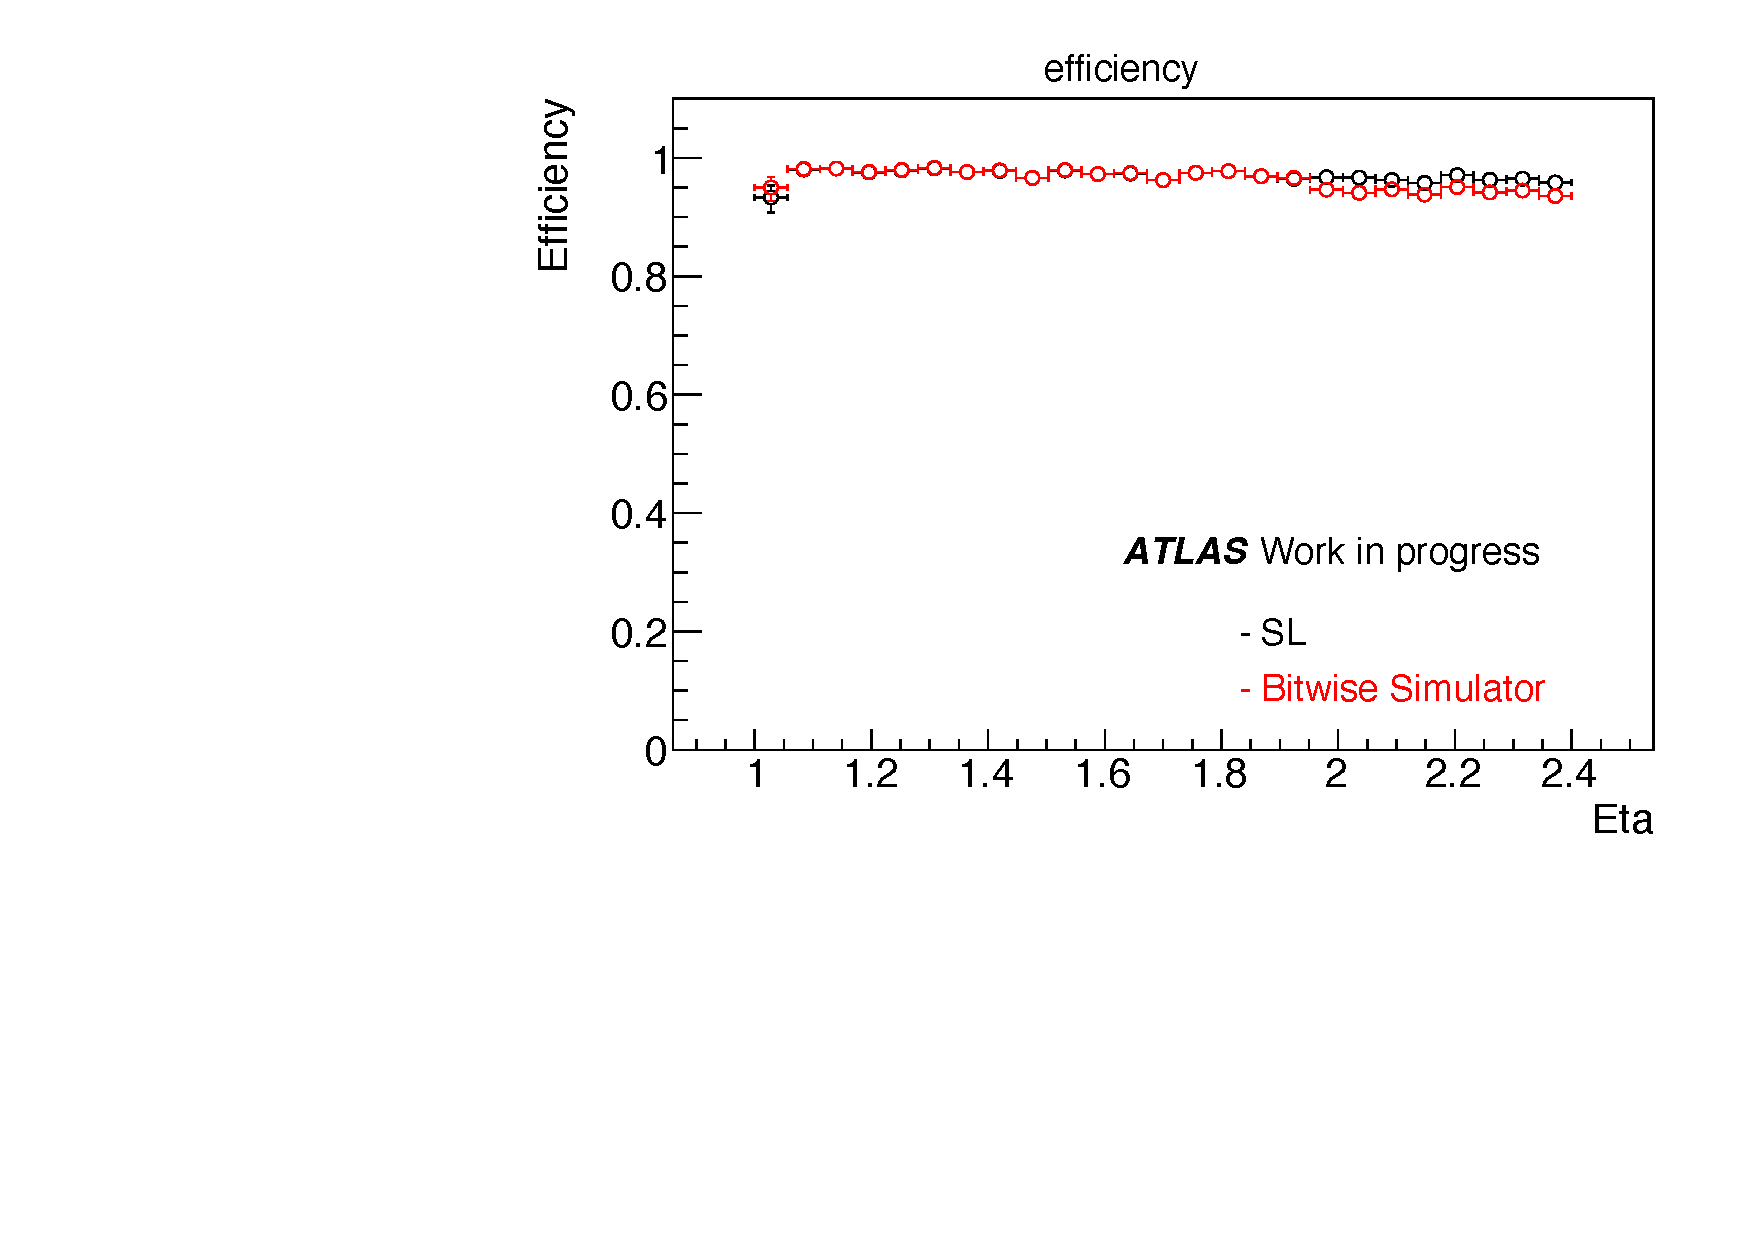
\includegraphics[height=10cm]{fig/Test/A_SM_strip_eta.pdf}
\subcaption{Strip Segment Reconstructino 検出効率の$\eta$依存性}
\end{minipage}\\
\begin{minipage}[b]{\linewidth}
\centering
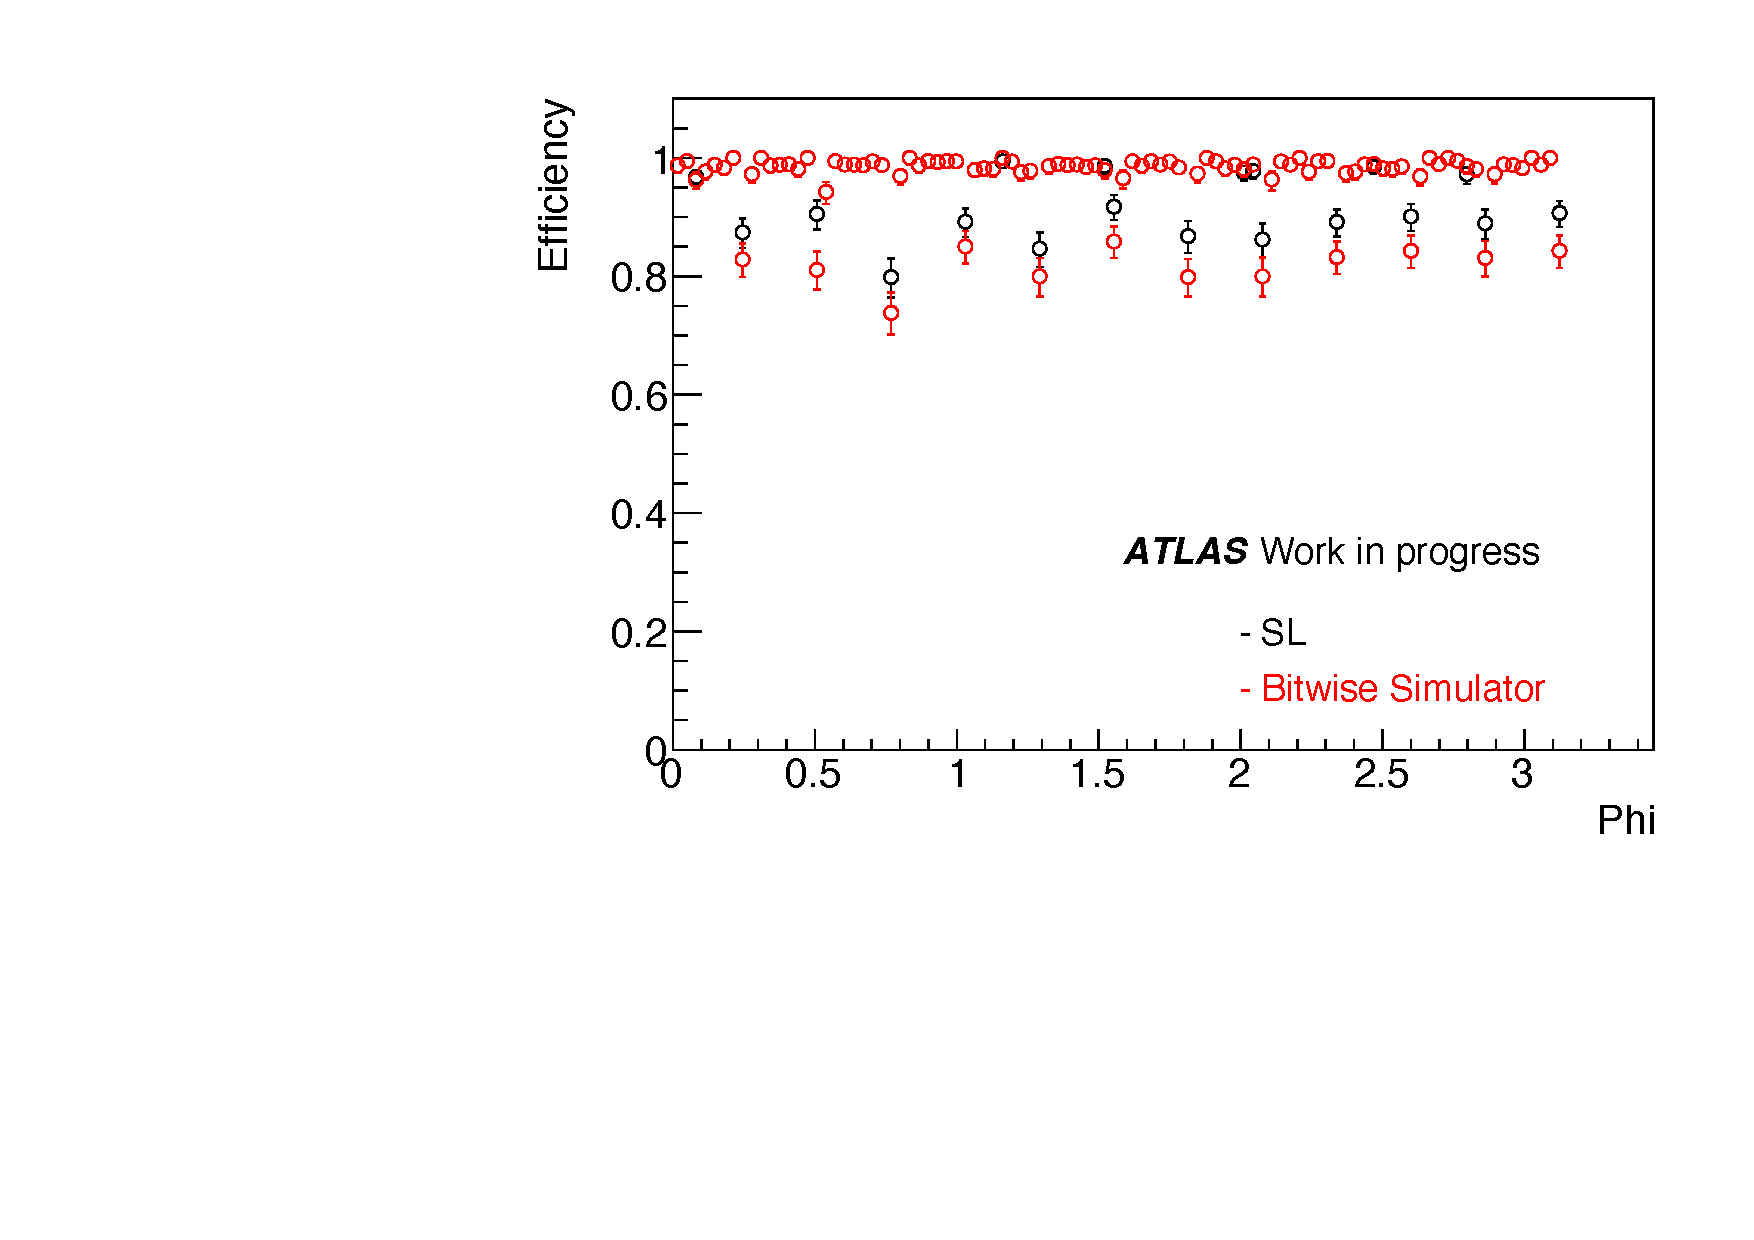
\includegraphics[height=10cm]{fig/Test/A_SM_strip_phi.pdf}
\subcaption{Strip Segment Reconstructino 検出効率の$\phi$依存性}
\end{minipage}%
\caption[Strip Segment Reconstructionの検出効率]{Strip Segment Reconstructionの検出効率}
\label{SM_A_strip}
\end{figure}



\subsubsection{Wire Segment Reconstruction}
\par
Stripの場合と同様に、Efficiencyは式\ref{eq:Wire_Efficiency}のように定義する。

\begin{equation}
    \mathrm {Efficiency} = \frac{\mathrm{Wire\,Segment \,Reconstruction\,で\Delta\eta\,を再構成できたイベント数}}{\mathrm{Truth\,pt \,20 \,GeV以上のイベント数}}
    \label{eq:Wire_Efficiency}
\end{equation}


Wire Segment Reconstructionの検出効率の$\eta$および$\phi$依存性を図\ref{SM_A_strip}に示す。$\eta$全領域での平均のトリガー効率は 96.3 \%であり、先行研究のVivadoシミュレーターの結果と矛盾しない結果が得られた。

トリガー効率の$\eta$依存性に着目すると、$\eta \sim 1.4$ 付近で約5 \%のInefficiencyが見られる。Bitwiseシミュレーターによる詳細な調査の結果、Station Coincidenceまでは期待通り動作しているものの、Segment ReconstructionでLUTから飛跡情報を取得できなかったため、飛跡再構成に失敗するイベントが発生していることが判明した。今後はLUTの修正を行い、この領域のInefficiencyを改善していく。

\begin{figure}
    \begin{minipage}[b]{\linewidth}
    \centering
    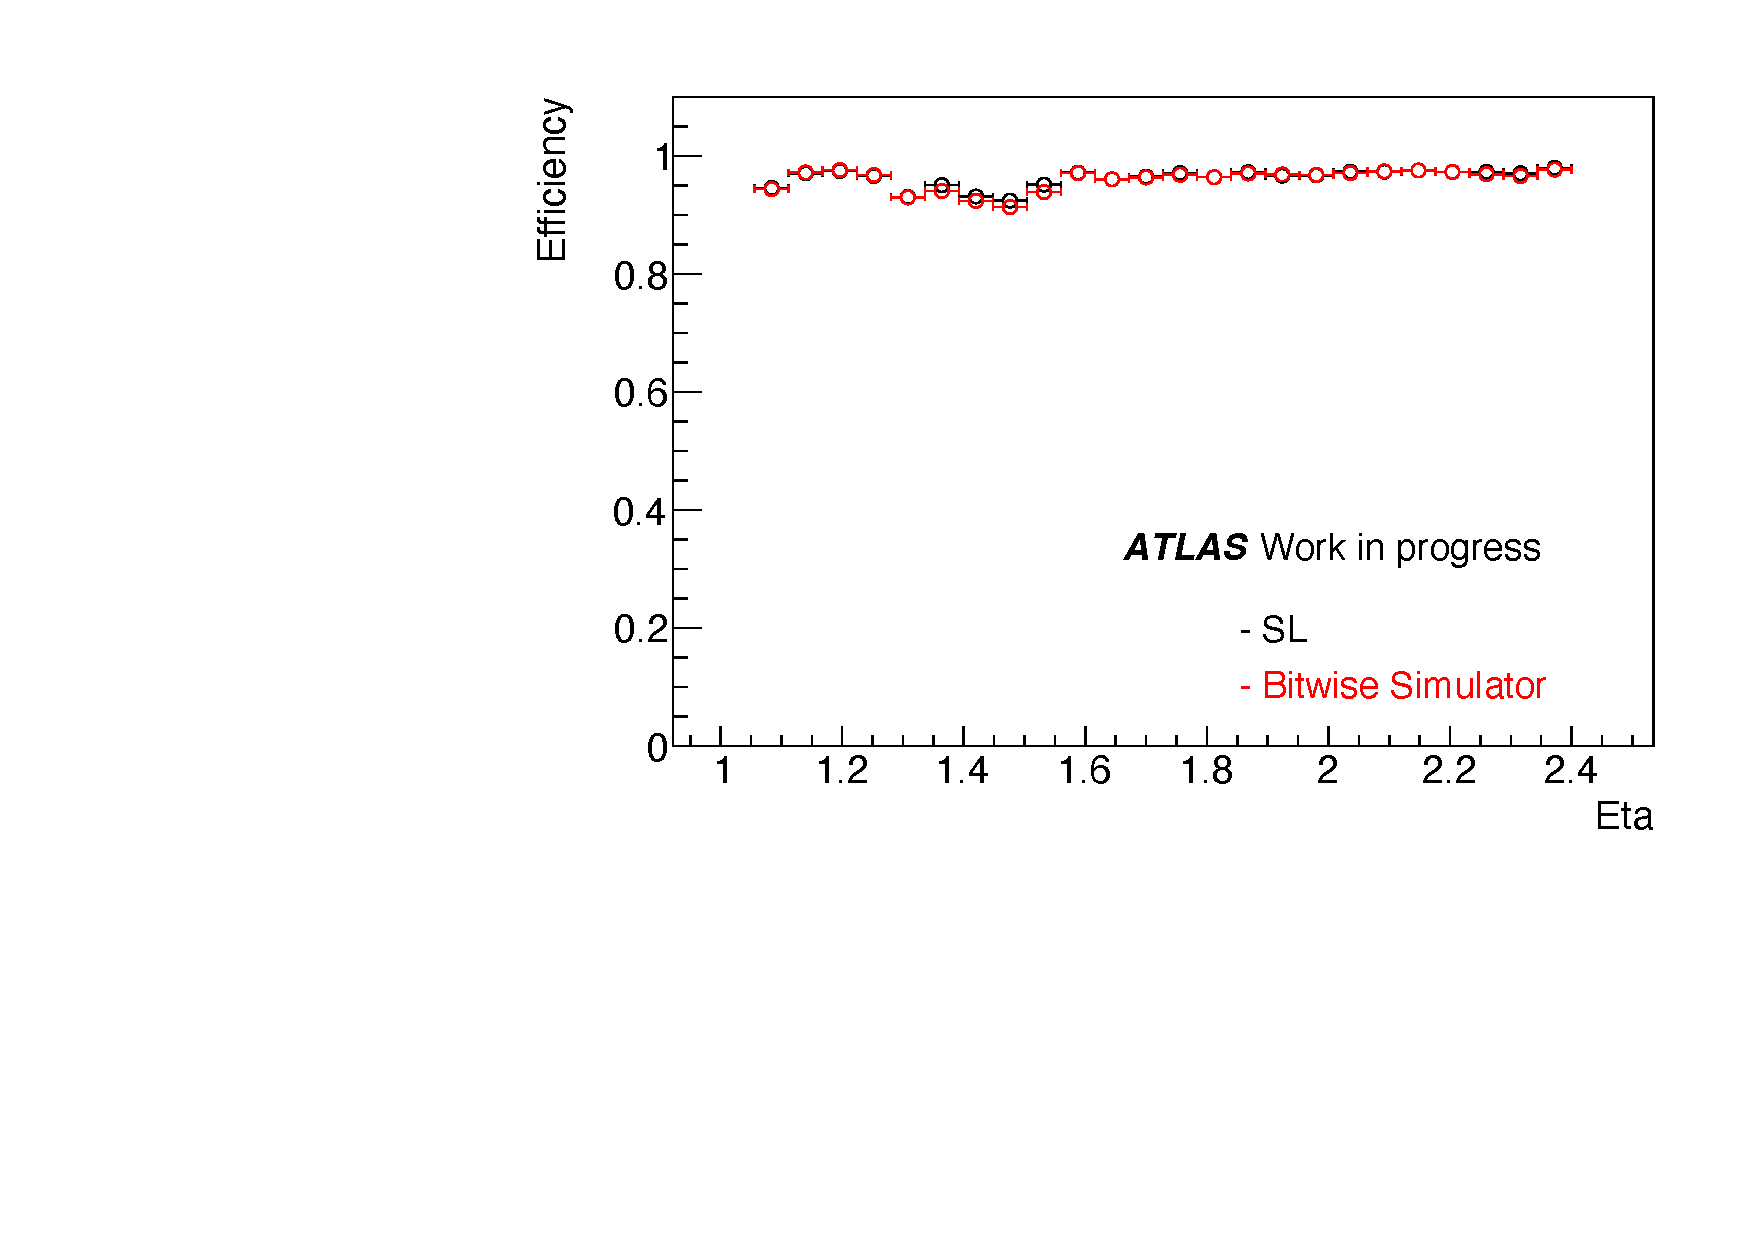
\includegraphics[height=10cm]{fig/Test/A_SM_wire_eta.pdf}
    \subcaption{Wire Segment Reconstructino 検出効率の$\eta$依存性}
    \end{minipage}\\
    \begin{minipage}[b]{\linewidth}
    \centering
    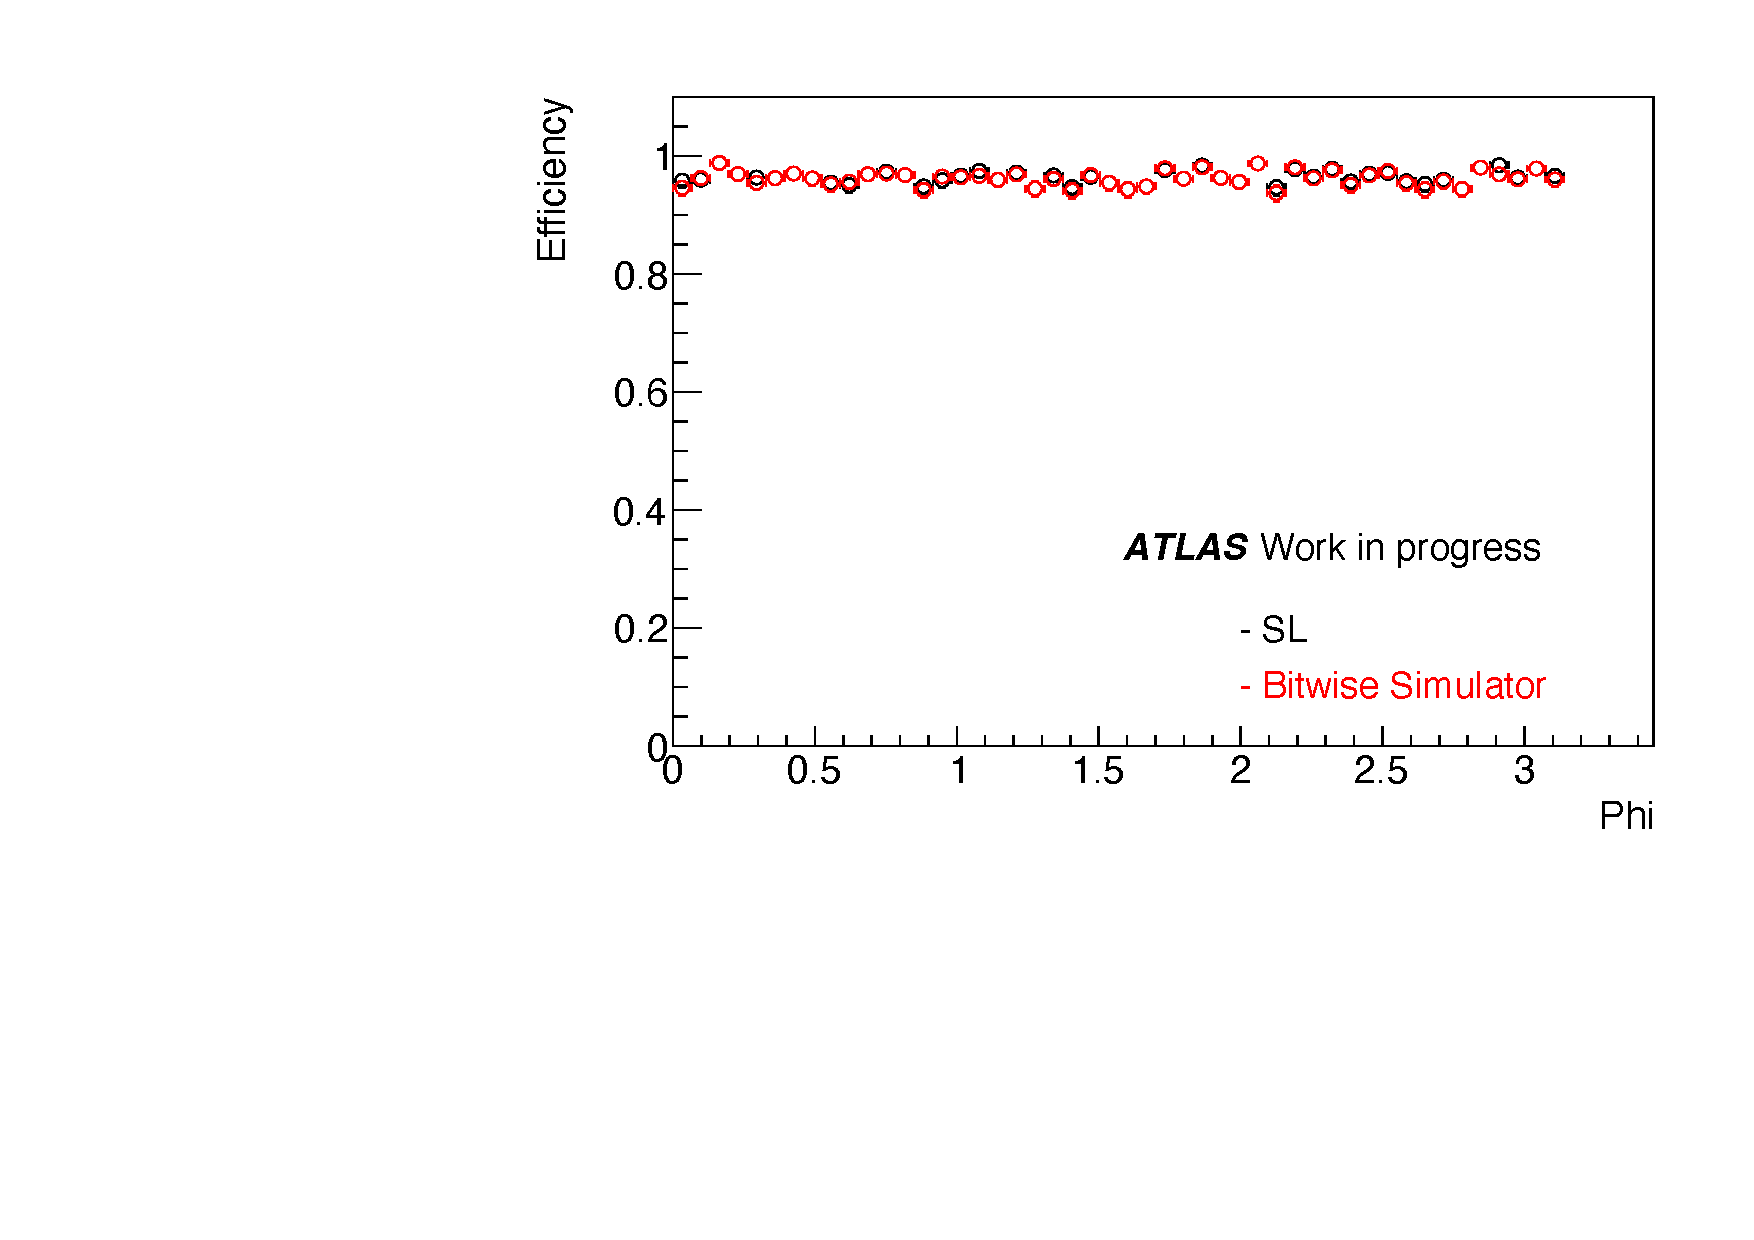
\includegraphics[height=10cm]{fig/Test/A_SM_wire_phi.pdf}
    \subcaption{Wire Segment Reconstructino 検出効率の$\phi$依存性}
    \end{minipage}%
    \caption[Wire Segment Reconstructionの検出効率]{Wire Segment Reconstructionの検出効率}
    \label{SM_A_Wire}
\end{figure}

\subsubsection{Wire Strip Coincidence}
Wire Strip Coincidenceは無限運動量飛跡を用いた試験で既にエンドキャップ領域に不具合が確認されているため、フォワード領域のみを評価することとする。またStripの試験で明らかになったチェンバー境界領域 ( チェンバーの両端から$\phi$方向に1割の領域 ) も除外し、不具合が確認されていない領域における検出効率を評価することを目的とする。ここではEfficiencyを式\ref{eq:WS_Efficiency}のように定義する。

\begin{equation}
    \mathrm {Efficiency} = \frac{\mathrm{Wire\,Strip\, Coincidenceで\,pt \,閾値\,20\,GeVと判定されたイベント数}}{\mathrm{Truth\,pt \,20 \,GeV以上のイベント数}}
    \label{eq:WS_Efficiency}
\end{equation}

図\ref{SM_A_WS}にWire Strip Coincidenceのフォワード領域検出効率の$\eta$依存性及び$\phi$依存性を示す。平均のトリガー効率は 93.5 \%であり、ソフトウェアシミュレーションの結果と矛盾のない結果が得られた。

\begin{figure}
    \begin{minipage}[b]{\linewidth}
    \centering
    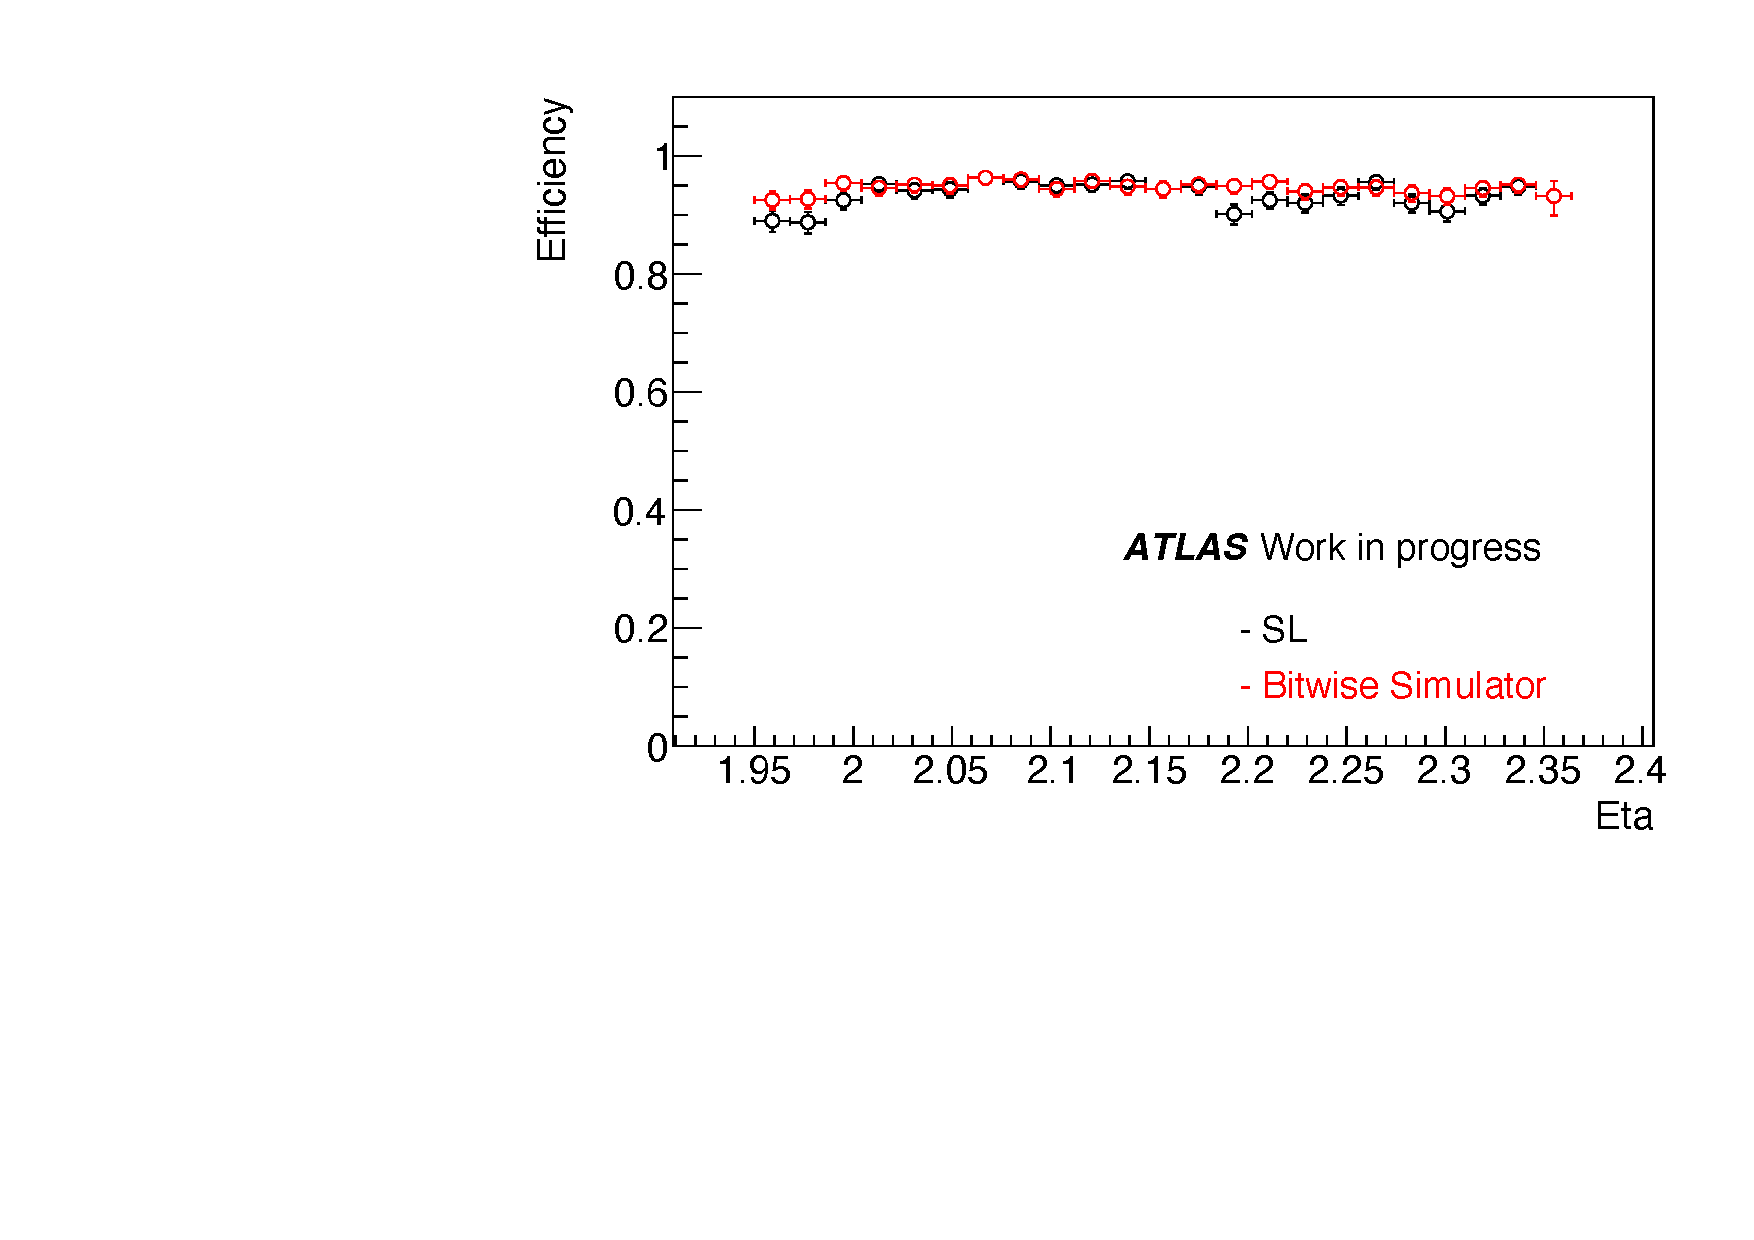
\includegraphics[height=10cm]{fig/Test/A_SM_ws_eta.pdf}
    \subcaption{Wire Strip Coincidence 検出効率の$\eta$依存性}
    \end{minipage}\\
    \begin{minipage}[b]{\linewidth}
    \centering
    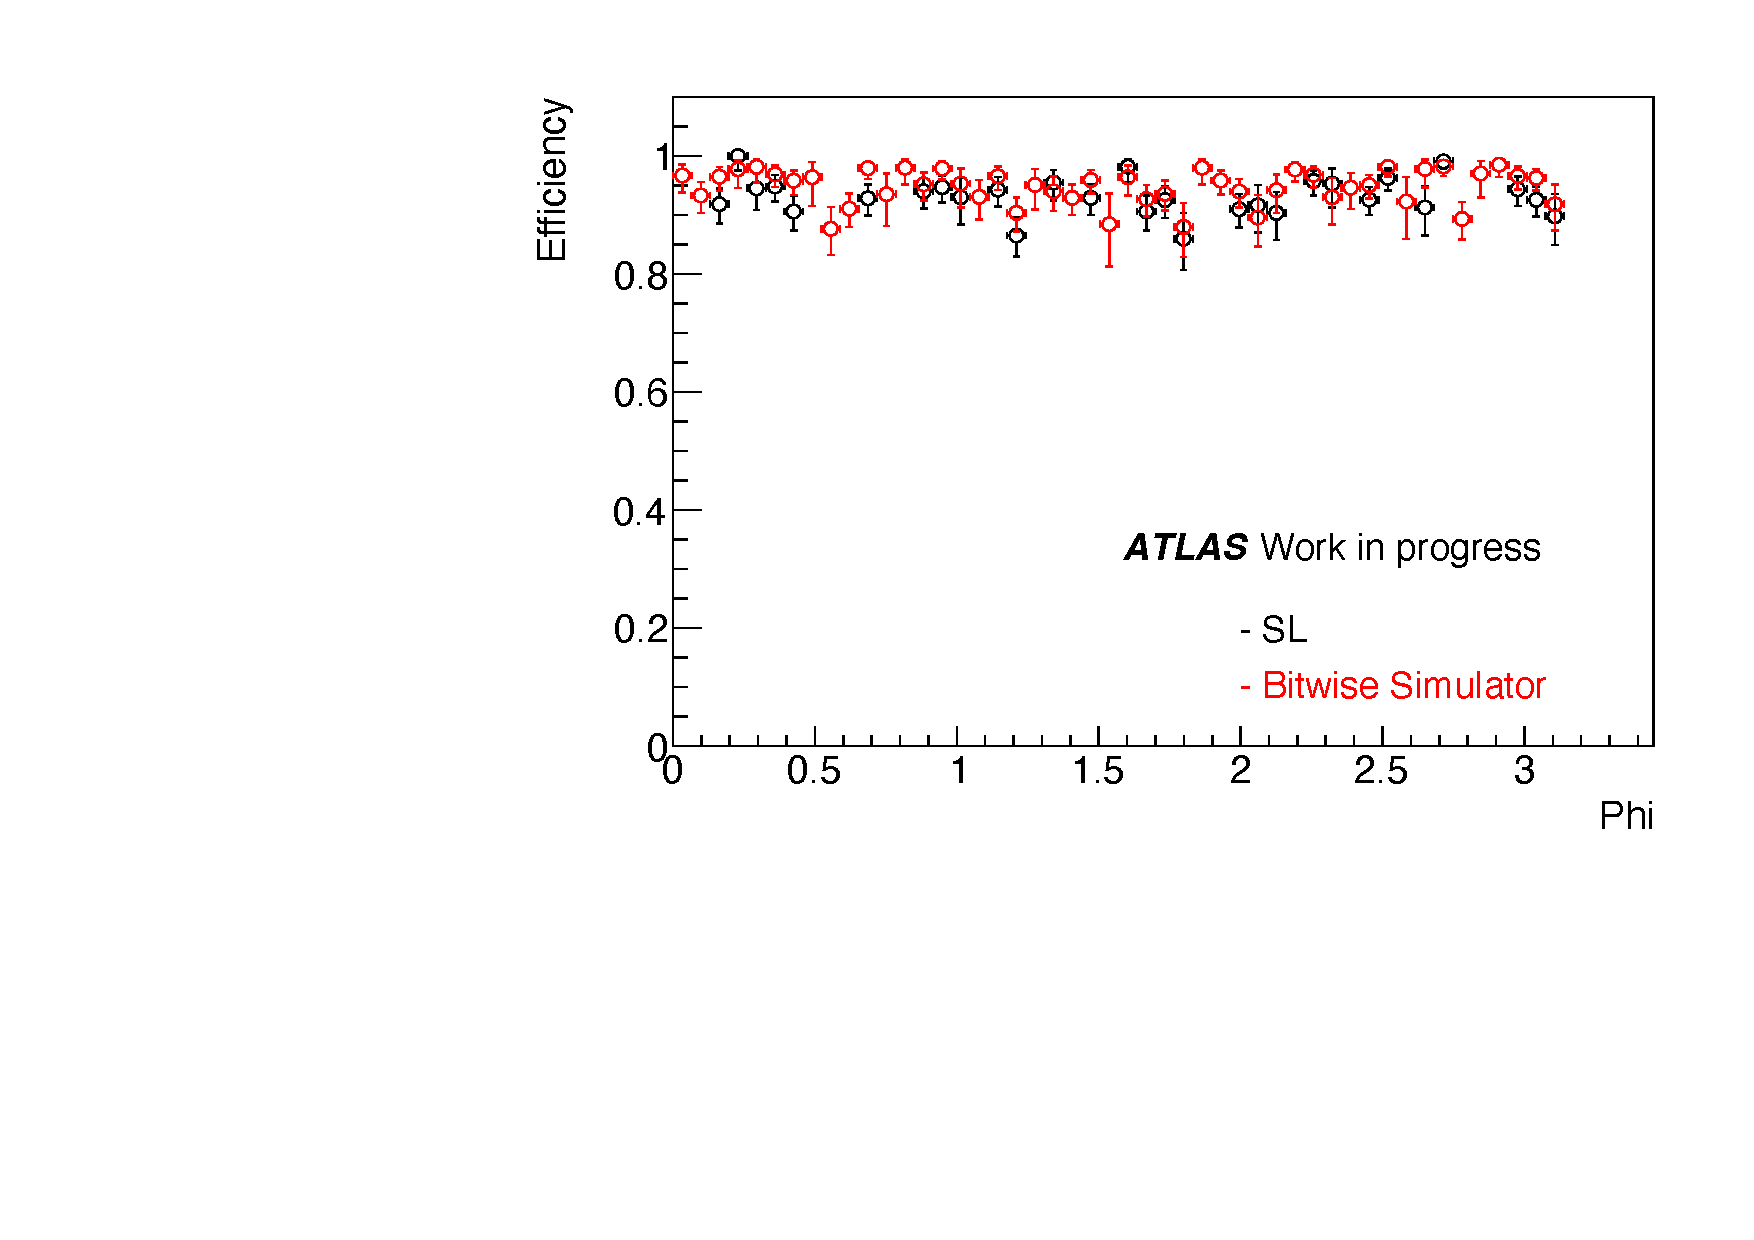
\includegraphics[height=10cm]{fig/Test/A_SM_ws_phi.pdf}
    \subcaption{Wire Strip Coincidence 検出効率の$\phi$依存性}
    \end{minipage}%
    \caption[Wire Strip Coincidenceの検出効率]{Wire Strip Coincidenceの検出効率}
    \label{SM_A_WS}
\end{figure}

図\ref{SM_A_WS_turnon}にはWire Strip Coincidenceの$p_\mathrm{T}$ごとの検出効率を示す。一般にこのような図をターンオンカーブという。赤色、青色、緑色、ピンクの各カーブは、それぞれがトリガー閾値20 GeV、15 GeV、10 GeV、5 GeVと判断されたイベントの割合を示している。どの\pt 閾値に対してもプラトー領域のefficiencyは93.5 \%程度であり、ソフトウェアシミュレーションやVivado シミュレーションの結果と一致している (図\ref{Soft_WS}) 。今後はエンドキャップ領域やチェンバー境界領域の不具合を解決し、全領域で期待されるパフォーマンスが得られるよう改善を続ける。

この結果を得るまでにWire Segment Reconstructionの問題点が発見され、修正が行われた。詳細をAppendix\ref{sec:appendix:MC-test}に記述する。また、プラトー領域に存在する6.5 \%程度のInefficiencyの原因についてもの調査を行った。この調査結果についてはAppendix\ref{sec:appendix:plateau}に詳細を記述する。
% さらに、今回の試験ではTGC検出器は理想位置と呼ばれる設計段階の位置に設置されていることを仮定して、モンテカルロデータやLUTを作成した。実験本番ではTGC検出器はアライメントの誤差により理想位置からずれた場所に設置される。このずれがトリガー効率にどれほど影響を与えるか調査した。その結果をAppendix{sec:appendix:alignment  \(\)}に示す。

\begin{figure} 
\centering
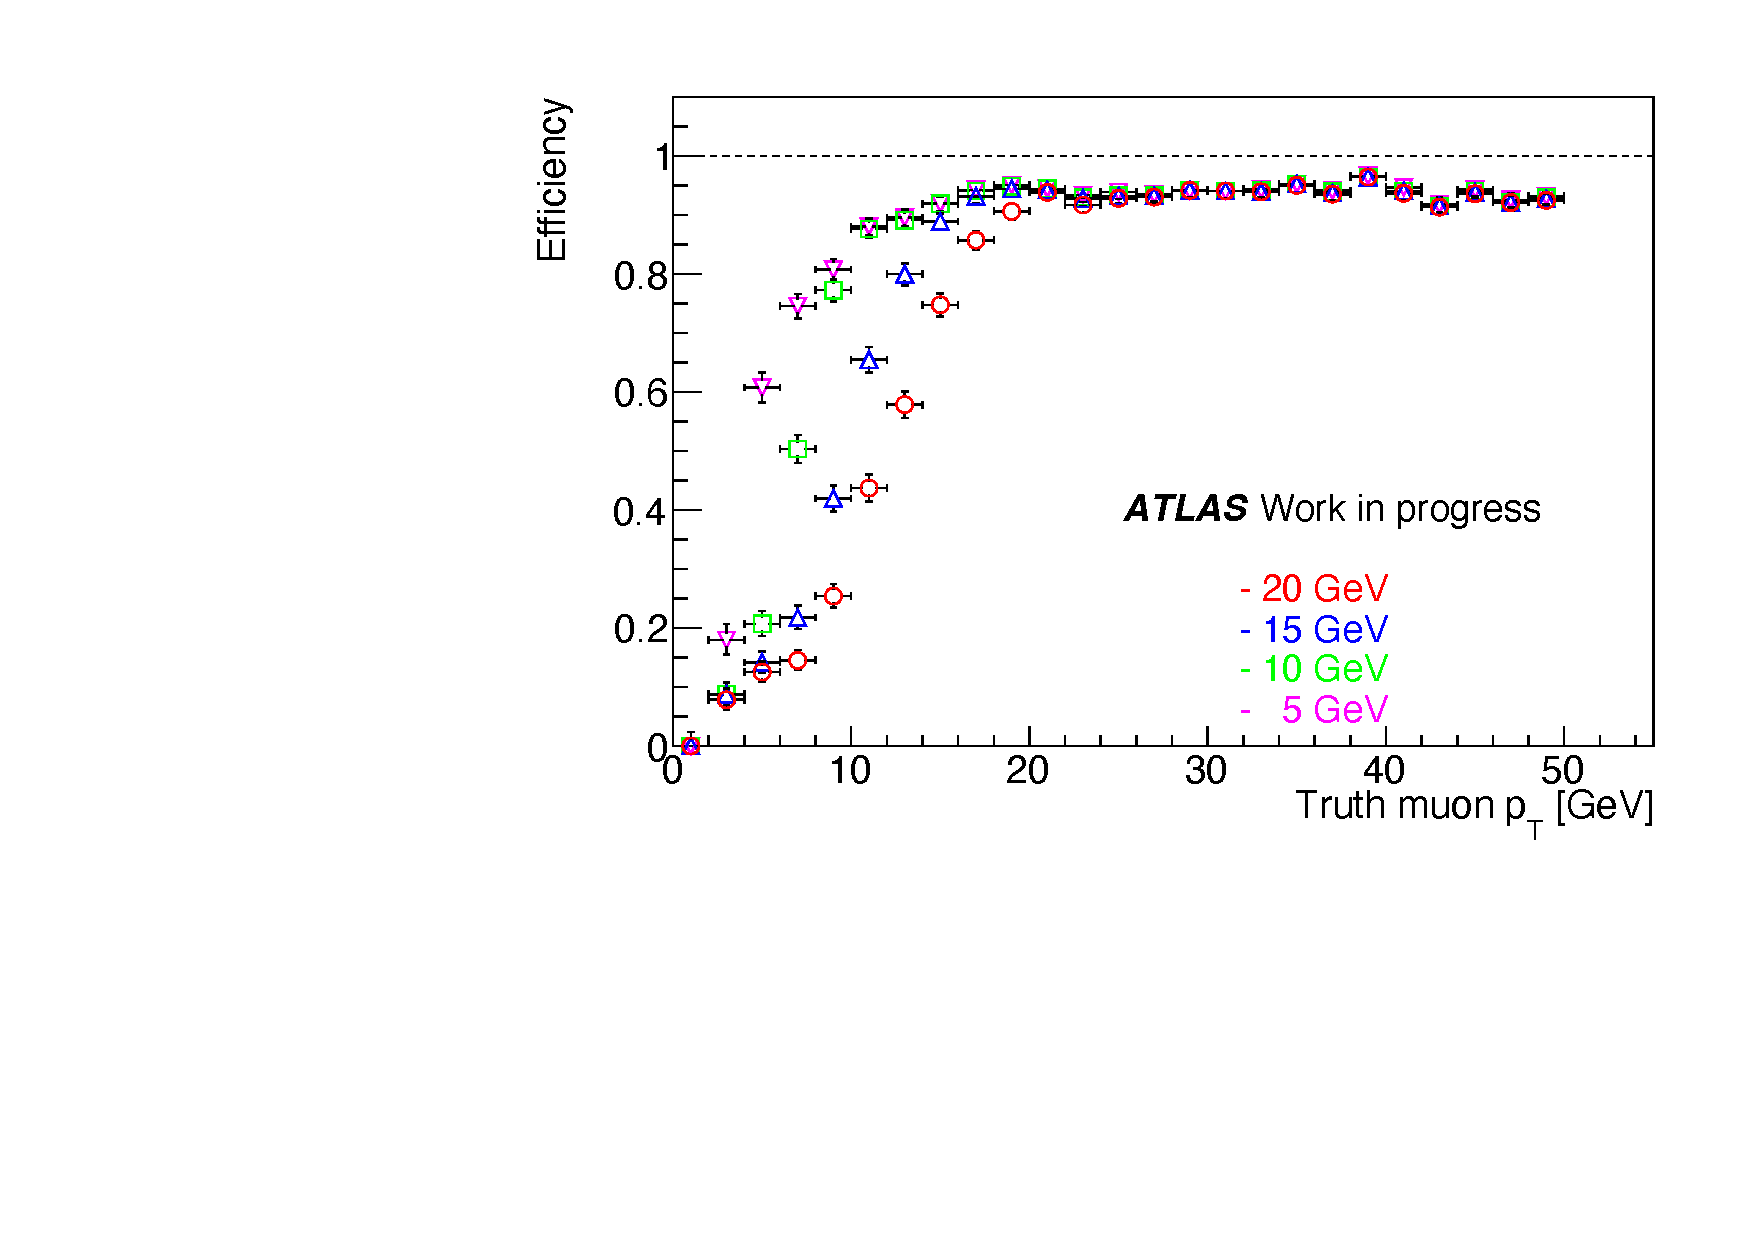
\includegraphics[width=16cm]{fig/Test/A_SM_ws_turnon.pdf}
\caption[]{Wire Strip Coincidenceの$p_\mathrm{T}$ごとの検出効率}
\label{SM_A_WS_turnon}
\end{figure}




